\chapter{Topology}
\section{Topological spaces}
\begin{propositionenv}
    Let $X$ be a set and for any $x\in X$, let $\mathcal{G}_x$ be a filter contained in the principal filter of $\{x\}$ ($\forall U\in \mathcal{G}_x,\ x\in U$). Denote by $\mathscr{T}$ the set 
    $$\{U\in \wp(X) \mid \forall x\in U, U\in\mathcal{G}_x\}.$$
    Then the following conditions are satisfied.
    \newline
    (1) $\{\varnothing, X\} \subseteq \mathscr{T}$.
    \newline
    (2) If $(U_1,U_2)\in \mathscr{T}^2$, then $U_1\cap U_2\in \mathscr{T}$.
    \newline
    (3) If $I$ is a set and $\left(U_i\right)_{i\in I}\in \mathscr{T}^I$, then $\dis \bigcup_{i\in I}U_i\in \mathscr{T}$.
    \newline
    Moreover, $\forall x\in X,\ \mathcal{B}_x=\{U\in \mathscr{T}\mid x\in U\}$ is a filter basis contained in $\mathcal{G}_x$. It generates $\mathcal{G}_x$ if the following condition is satisfied:
    $$\forall U\in \mathcal{G}_x,\ \exists V\in \mathcal{G}_x,\ V\subseteq U \text{ and } \forall y\in V,\ V\in \mathcal{G}_y.$$
\end{propositionenv}
\begin{proofenv}
    \ \newline
    (1) $\dis \varnothing \in \mathscr{T}, X\in \bigcap_{x\in X}\mathcal{G}_x$.
    \newline
    (2) $\forall x\in U_1\cap U_2,\ U_1\in \mathcal{G}_x,\ U_2\in \mathcal{G}_x$, so $U_1\cap U_2\in \mathcal{G}_x$.
    \newline
    (3) Let $\dis U=\bigcup_{i\in I}U_i$. $\forall x\in U,\ \exists i\in I,\ x\in U_i$, so $U_i\in \mathcal{G}_x$. Since $U\supseteq U_i$, so $U\in\mathcal{G}_x$.
    $$\mathcal{B}_x:=\{U\in \mathscr{T}\mid x\in U\}.$$
    If $U\in \mathcal{B}_x$, then $x\in U$, so $U\in \mathcal{G}_x$. Hence $\mathcal{B}_x\subseteq\mathcal{G}_x$. If $(U,V)\in \mathcal{B}_x^2$, then $U\cap V\in \mathscr{T}$, and $x\in U\cap V$. So $U\cap V\in \mathcal{B}_x$. So $\mathcal{B}_x$ is a filter basis. Suppose the condition is satisfied. For any $U\in \mathcal{G}_x,\ \exists V\in \mathcal{G}_x\cap\mathscr{T}$, such that $V\subseteq U$. Note that $V\in \mathcal{B}_x$, so $\mathcal{G}_x$ is generated by $\mathcal{B}_x$.
\end{proofenv}
\begin{definitionenv}
    Let $X$ be a set. We call \textbf{topology} on $X$ any subset $\mathscr{T}$ of $\wp(X)$ that satisfies the following conditions:
     \newline
    (1) $\{\varnothing, X\} \subseteq \mathscr{T}$.
    \newline
    (2) If $(U_1,U_2)\in \mathscr{T}^2$, then $U_1\cap U_2\in \mathscr{T}$.
    \newline
    (3) For any set $I$,  $ \forall \left(U_i\right)_{i\in I}\in \mathscr{T}^I$, then $\dis \bigcup_{i\in I}U_i\in \mathscr{T}$.
    \newline
    $(X,\mathscr{T})$ is called a \textbf{topological space}.
    \newline
    If $\forall x\in X,\ \mathcal{B}_x$ is a filter basis of $X$ contained in the principal filter of $\{x\}$, then 
    $$\mathscr{T}=\{U\in \wp(X)\mid \forall x\in U,\ \exists V_x\in \mathcal{B}_x,\ V_x\subseteq U\}$$
    is a topology on $X$, called the \textbf{topology generated by} $(\mathcal{B}_x)_{x\in X}$. More generally, if $\forall x\in X,\ S_x $ is a subset of the principal filter of $\{x\}$ and $\mathcal{G}_x$ is the filter generated by $S_x$, then we say that 
    $$\mathscr{T}=\{U\in\wp(X)\mid \forall x\in U,\ U\in \mathcal{G}_x\}$$
    is the topology generated by $(S_x)_{x\in X}$.

\end{definitionenv}
\begin{exampleenv}
    \ \newline
    (1) Let $\mathcal{G}_x=\{X\}$. The topology generated by $\left(\mathcal{G}_x\right)_{x\in X}$ is $\{\varnothing,X\}$, called the \textbf{trivial topology} on $X$.  
    \newline
    (2) Let $\mathcal{G}_x=\mathcal{F}_{\{x\}}$ be the principal filter. The topology generated by $\left(\mathcal{G}_x\right)_{x\in X}$ is $\wp(X)$. This topology is called the \textbf{discrete topology} on $X$.
    \newline
    (3) Let $(X,\mathrm{d})$ be a semimetric space. 
    $$\mathrm{d}:X\times X\longrightarrow \mathbb{R}_{\ge 0},\  \mathrm{d}(x,y)=\mathrm{d}(y,x),\ \mathrm{d}(x,z)\le \mathrm{d}(x,y)+\mathrm{d}(y,z),\ \mathrm{d}(x,x)=0.$$
    $\forall \varepsilon>0,\ \forall x\in X$, let $B(x,\varepsilon)=\{y\in X\mid \mathrm{d}(x,y)<\varepsilon\}$, $\{B(x,\varepsilon)\mid \varepsilon\in \RR_{>0}\}=: \mathcal{B}_x$ is a filter basis on $X$, $\mathcal{B}_x$ is contained in the principal filter of $\{x\}$. The topology 
    $$\mathscr{T}=\{U\in \wp(X)\mid \forall x\in U,\ \exists \varepsilon\in \RR_{>0},\ B(x,\varepsilon)\subseteq U\}$$
    is called the \textbf{topology induced by the semimetric $\mathrm{d}$}.
    \newline
    (4) Let $(G,\le )$ be a totally ordered set $\forall x\in G$, let $S_x=\{G_{>a}\mid a<x\}\cup \{G_{<b}\mid x<b\}$
\end{exampleenv}
\begin{propositionenv}
    $\forall x\in X,\ \forall \varepsilon\in \RR_{>0}, B(x,\varepsilon)\in \mathscr{T}$.
\end{propositionenv}
\begin{proofenv}
    $\forall y\in B(x,\varepsilon),\ \mathrm{d}(x,y)<\varepsilon$. Let $r=\varepsilon-\mathrm{d}(x,y)>0$, we claim that $B(y,r)\subseteq B(x,\varepsilon)$. Let $z\in B(y,r), \ \mathrm{d}(y,z)<r$. Hence,
    $$\mathrm{d}(x,z)\le \mathrm{d}(x,y)+\mathrm{d}(y,z)<\mathrm{d}(x,y)+r=\mathrm{d}(x,y)+\varepsilon -\mathrm{d}(x,y)=\varepsilon.$$
\end{proofenv}
\begin{remark}
    On $\RR$, one has a metric 
    $$\mathrm{d}: \RR\times \RR\longrightarrow \RR_{\ge 0},$$
    $$\left(a,b\right)\longmapsto |a-b|.$$
    $$B(x,\varepsilon)=\interval[open]{x-\varepsilon}{x+\varepsilon}.$$
    $$\mathcal{B}_x=\{\interval[open]{x-\varepsilon}{x+\varepsilon}\mid \varepsilon\in \RR_{>0}\}.$$
    Let $\mathscr{T}_\mathrm{d}$ be the topology generated by $(\mathcal{B}_x)_{x\in \RR}$. Let $\mathscr{T}$ be the order topology generated by $\left(S_x\right)_{x\in \RR}$, where 
    $$S_x:=\{\RR_{>a}\mid a<x\}\cup \{\RR_{<b}\mid x<b\}.$$
\end{remark}
\begin{propositionenv}
    For any $x\in \RR$, $\mathcal{F}(\mathcal{B}_x)=\mathcal{F}(S_x)$.
\end{propositionenv}
\begin{proofenv}
    $\forall \varepsilon>0,\ \interval[open]{x-\varepsilon}{x+\varepsilon}=\RR_{<x+\varepsilon}\cap \RR_{>x-\varepsilon}\in \mathcal{F}(S_x)$. So $\mathcal{F}(\mathcal{B}_x)\subseteq \mathcal{F}(S_x)$.
    $$\forall a\in \RR,\ a<x,\ \RR_{>a}\supseteq \interval[open]{a}{2x-a}=\interval[open]{x-(x-a)}{x+(x-a)},\ \RR_{>a}\in \mathcal{F}(\mathcal{B}_x).$$
    $$\forall b\in \RR, b>x,\RR_{<b}\supseteq \interval[open]{2x-b}{b}=\interval[open]{x+(b-x)}{x+(b-x)},$$
    So, $\RR_{<b}\subseteq\mathcal{F}(\mathcal{B}_x)$. Hence $S_x\subseteq \mathcal{F}(\mathcal{B}_x)$, which leads to $\mathcal{F}(S_x)\subseteq\mathcal{F}(\mathcal{B}_x)$.
\end{proofenv}
\begin{definitionenv}
    Let $(X,\mathscr{T})$ be a topological space. For any $x\in X$ and any $V\in \wp(X)$, if there exists $U\in \mathscr{T}$ such that $x\in U\subseteq V$, then we say that $V$ is a \textbf{neighborhood of $x$}. We call \textbf{open subset} of $X$ any subset of $X$ that belongs to $\mathscr{T}$. If $U\in \mathscr{T}$, such that $x\in U$, we say that $U$ is an \textbf{open neighborhood of $x$}. We denote by $\mathcal{V}_x(\mathscr{T})$ the set of all neighborhoods of $x$.
\end{definitionenv}
\begin{propositionenv}
    $\mathcal{V}_x(\mathscr{T})$ is a filter on $X$ contained in the principal filter of $\{x\}$. Moreover, the topology generated by $\left(\mathcal{V}_x(\mathscr{T})\right)_{x\in X}$ identifies with $\mathscr{T}$.
\end{propositionenv}
\begin{proofenv}
    \ \newline
    (1) If $(V_1,V_2)\in \mathcal{V}_x(\mathscr{T})^2,\ \exists (U_1,U_2)\in \mathscr{T}^2$, such that $x\in U_1\subseteq V_1,\ x\in U_2\subseteq V_2$. Hence, $x\in U_1\cap U_2\subseteq V_1\cap V_2$, so $V_1\cap V_2\in \mathcal{V}_{x}(\mathscr{T})$.
    \newline
    (2) If $V\in \mathcal{V}_x(\mathscr{T})$, $W\in \wp(X),\ V\subseteq W$. $\exists U\in \mathscr{T}$, $x\in U\subseteq V\subseteq W$, so $W\in \mathcal{V}_x(\mathscr{T})$. Let $\mathscr{T}'$ be the topology generated by $\left(\mathcal{V}_x(\mathscr{T})\right)_{x\in X}$. By definition,
    $$\mathscr{T}'=\{U\subseteq X\mid \forall x\in U, U\in \mathcal{V}_x(\mathscr{T})\}.$$
    For any $U\in \mathscr{T},\ \forall x\in U  $, $U$ is a open neighborhood of $x$, so $U\in \mathscr{T}'$. Let $U\in \mathscr{T}', \ \forall x\in U,\ \exists V_2\in \mathscr{T},\ x\in V_x\subseteq U$.
    $$U=\bigcup_{x\in U}\{x\}\subseteq \bigcup_{x\in U}V_x\subseteq U.$$
    $$U=\bigcup_{x\in U}V_x\in \mathscr{T}.$$
\end{proofenv}
\begin{propositionenv}
    Let $X$ be a set, $\left(\mathscr{T}_i\right)_{i\in I}$ be a family of topologies on $X$. Then 
    $$\mathscr{T}=\bigcap_{i\in I}\mathscr{T}_i$$
    is a topology on $X$.
\end{propositionenv}
\begin{proofenv}
    \ \newline
    (1) $\forall i\in I,\ \{\varnothing,X\}\subseteq \mathscr{T}_i$, so $\{\varnothing,X\}\subseteq \mathscr{T}$.
    \newline
    (2) If $(U_1,U_2)\in \mathscr{T}^2$, then for any $i\in I$, $\ U_1\cap U_2\in \mathscr{T}_i$, so $\dis U_1\cap U_2\in \bigcap_{i\in I}\mathscr{T}_i$.
    \newline
    (3) For any set $J$ and any $\left(U_j\right)_{j\in J}\in \mathscr{T}^J$, one has $\forall i\in I,\ \forall j\in J,\ U_j\in \mathscr{T}_i$, so
    $$\bigcup_{j\in J}U_j\in \mathscr{T}_i.$$
    Therefore, $$\bigcup_{j\in J}U_j\in \bigcap_{i\in I}\mathscr{T}_i.$$ 
\end{proofenv}
\begin{definitionenv}
    Let $S$ be a subset of $\wp(X)$, we denote by $\mathscr{T}_S$ the intersection of all topologies containing $S$, we call it the topology generated by $S$. 
\end{definitionenv}
\begin{definitionenv}
    \ \newline
    Let $\mathcal{B}$ be a subset of $\wp(X)$, we say that $\mathcal{B}$ is a \textbf{topological basis} if:
    \newline
    (1) $\dis X=\bigcup_{V\in \mathcal{B}}V$.
    \newline
    (2) $\forall (U,V)\in \mathcal{B}\times\mathcal{B},\ \forall x\in U\cap V,\ \exists W_x\in \mathcal{B},\ x\in W_x\subseteq U\cap V$.
\end{definitionenv}
\begin{definitionenv}
    Let $X$ be a set and $\mathscr{T}_1$ and $\mathscr{T}_2$ be two topologies on $X$. If $\mathscr{T}_1\subseteq\mathscr{T}_2$, we say that $\mathscr{T}_1$ is coarser than $\mathscr{T}_2$ and $\mathscr{T}_2$ is finer than $\mathscr{T}_1$. 
    
    If $S\subseteq\wp(X)$, we denote by $\mathscr{T}_S$ the intersection of all topology containing $S$. It is the coarsest topology containing $S$. 
    
\end{definitionenv}
\begin{propositionenv}
    Let $S$ be s subset of $\wp(X)$. Let 
    $$\mathcal{B}_S:=\{X\}\cup\left\{\bigcap_{i=1}^{n}A_i\mid n\in \NN_{\ge 1},\ (A_1,\dots,A_n)\in S^n\right\},$$
    then, $\mathcal{B}_S$ is a topological basis on $X$. Moreover, $\mathscr{T}_S=\mathscr{T}_{\mathcal{B}_S}$.
\end{propositionenv}
\begin{proofenv}
    Since $X\in \mathcal{B}_S$, $\dis\bigcup_{V\in \mathcal{B}_S}V=X$. Let $(U,V)\in \mathcal{B}_S\times\mathcal{B}_S$. If $U=X$, then $U\cap V=V\in \mathcal{B}_S$. Similarly, if $V=X$, then $U\cap V=U\in \mathcal{B}_S$. 

    If $U=A_1\cap\dots\cap A_n,\ V=B_1\cap\dots\cap B_m$, then $\{A_1,\dots, A_n,B_1,\dots,B_m\}\subseteq \mathcal{B}_S$. 
    $$U\cap V=A_1\cap\dots\cap A_n\cap B_1\cap\dots\cap B_m\in \mathcal{B}_S.$$
    Since $S\subseteq\mathcal{B}_S\subseteq\mathscr{T}_{\mathcal{B}_S}$, so $\mathscr{T}_{S}\subseteq\mathscr{T}_{\mathcal{B}_S}, \ X\in \mathscr{T}_S$. If $(A_1,\dots,A_n)\in S^n$, then $(A_1,\dots,A_n)\in\mathscr{T}_{\mathcal{B}_S}$. So $A_1\cap\dots\cap A_n\in \mathscr{T}_S$. Hence $\mathcal{B}_S\subseteq\mathscr{T}_{S}$. Therefore, $\mathscr{T}_{\mathcal{B}_S}\subseteq\mathscr{T}_S$, so $\mathscr{T}_{\mathcal{B}_S}=\mathscr{T}_S$.
\end{proofenv}
\begin{propositionenv}
    Let $\mathcal{B}$ be a topological basis on a set $X$. Then
    $$\mathscr{T}_{\mathcal{B}}=\left\{U\in\wp(X)\mid \exists \text{ a set }I \text{ and }(V_i)_{i\in I}\in \mathcal{B}^I, U=\bigcup_{i\in I}V_i\right\}.$$
\end{propositionenv}
\begin{proofenv}
    We denote by $\mathscr{T}$ the set 
    $$\{U\in \wp(X)\mid U\text{ can be written as as the union of a family sets in }\mathcal{B}\}.$$
    By definition, $\mathcal{B}\subseteq\mathscr{T}\subseteq\mathscr{T}_{\mathcal{B}}$. It remains to check that $\mathscr{T}$ is a topology.

    By definition, $X\in \mathscr{T},\ \varnothing\in \mathscr{T}$. Moreover, the union of a family of elements of $\mathscr{T}$ remains in $\mathscr{T}$. Let $\dis U=\bigcup_{i\in I}U_i$ and $\dis V=\bigcup_{j\in J}V_j$ be elements of $\mathscr{T}$, where, $U_i\in\mathcal{B}, V_{j}\in \mathcal{B}$. Then 
    $$ U\cap V=\bigcup_{(i,j)\in I\times J}\left(U_i\cap V_{j}\right).$$
    For any $x\in U_i\cap V_j$, $\exists W_x^{(i,j)}\in \mathcal{B},\ x\in W_x^{(i,j)}\subseteq U_i\cap V_j$. $\dis U_i\cap V_j=\bigcup_{x\in U_i\cap V_j}W_x^{(i,j)}$, so 
    $$U\cap V=\bigcup_{(i,j)\in I\times J}\bigcup_{x\in U_i\cap V_j}W_x^{(i,j)}.$$
\end{proofenv}


\section{Convergence}
We fix a topology space $(E,\mathscr{T})$, $l\in E$ and $S\subseteq \wp(E)$ that generates the filter $\mathcal{V}_l(\mathscr{T})$ of all neighborhood  of $l$.
\begin{definitionenv}
    Let $f:X\longrightarrow Y$ be a mapping. If $\mathcal{F}$ is a filter on $X$, we denote by $f_*(\mathcal{F})$ the set $\{B\subseteq Y\mid f^{-1}(B)\in\mathcal{F}\}$. 
\end{definitionenv}
\begin{propositionenv}
    $f_*(\mathcal{F})$ is a filter on $Y$.
\end{propositionenv}
\begin{proofenv}
    Let $(B_1,B_2)\in f_*(\mathcal{F})$,
    $$f^{-1}(B_1\cap B_2)=f^{-1}(B_1)\cap f^{-1}(B_2)\in \mathcal{F}.$$
    Let $B\in f_*(\mathcal{F}),\ C\supseteq B$. $f^{-1}(C)\supseteq f^{-1}(B)\in\mathcal{F}$, so $f^{-1}(C)\in \mathcal{F}$.
\end{proofenv}
\begin{propositionenv}
    Let $f:X\longrightarrow Y, \ g:Y\longrightarrow Z$, be mappings. $\mathcal{F}$ be a filter on $X$. Then
    $$\left(g\circ f\right)_{*}(\mathcal{F})=g_*(f_*(\mathcal{F})).$$
\end{propositionenv}
\begin{proofenv}
    \begin{align*}
        \left(g\circ f\right)_*(\mathcal{F})=&\{C\subseteq Z\mid \left(g\circ f\right)^{-1}(C)\in\mathcal{F}\}\\
        =&\{C\subseteq Z\mid f^{-1}(g^{-1}(C))\in \mathcal{F}\}\\
        =&\{C\subseteq Z\mid g^{-1}(C)\in f_*(\mathcal{F})\}\\
        =&g_*(f_*(\mathcal{F})).
    \end{align*}
\end{proofenv}
\begin{propositionenv}
    Let $\mathcal{B}$ be a filter basis in $X$,  $f:X\longrightarrow Y$ be a mapping and $\mathcal{F}$ be the filter generated by $\mathcal{B}$. Then $f(\mathcal{B}):\{f(U)\mid U\in \mathcal{B}\}$  is a filter basis on $Y$ and $f_*(\mathcal{F})$ is the filter generated by $f(\mathcal{B})$.
\end{propositionenv}
\begin{proofenv}
    Let $U$ and $V$ be elements of $\mathcal{B}$. Then $\exists W\in \mathcal{B},\ W\subseteq U\cap V$. Hence $f(W)\subseteq f(U\cap V)\subseteq f(U)\cap f(V).$ Moreover, for any $U\in\mathcal{B}$, $U\subseteq f^{-1}(f(U))$. So $f^{-1}(f(U))\in \mathcal{F}$. Therefore, $f(\mathcal{B})\subseteq f_*(\mathcal{F}) $. Let $A\in f_*(\mathcal{F})$. Then, $f^{-1}(A)\in \mathcal{F}$. So $\exists V\in \mathcal{B},\ V\subseteq f^{-1}(A)$. Hence $f(V)\subseteq A$. Therefore, $f_*(\mathcal{F})$ is a filter basis generated by $f_*(\mathcal{B})$
\end{proofenv}
\begin{definitionenv}
    Let $f:X\longrightarrow E$ be a mapping, $\mathcal{F}$ be a non-degenerate filter on $X$. If $f_*(\mathcal{F})\supseteq \mathcal{V}_l(\mathscr{T})$, we say that $f$ \textbf{converges} to $l$ along $\mathcal{F}$.
    $$\lim_{\mathcal{F}}f=l $$
    denotes ``$f$ converges to $l$ along $\mathcal{F}$''.

    This condition is equivalent to 
    $$\forall V\in S_l,\ f^{-1}(V)\in \mathcal{F}.$$
    If $\mathcal{B}$ is a filter basis which generates $\mathcal{F}$. This condition is also 
    $$\forall V\in S_l,\ \exists U\in \mathcal{B},\ f(U)\subseteq V.$$
    
\end{definitionenv}
\begin{exampleenv}
    \ \newline
    (1) Let $I\subseteq \NN$ be an infinite subset and $x=(x_n)_{n\in I}\in \NN^I$. Let $\mathcal{F}$ be the Fréchet filter on $I$. If $x$ converges to $l$ along $\mathcal{F}$, or equivalently,
    $$\forall V\in S_l,\ \exists N\in \NN,\ \forall n\in I_{\ge \NN},\ x_n\in V.$$
    We say that the sequence $(x_n)_{n\in I}$ \textbf{converges to $l$} when $n$ tends to the infinity, denote as 
    $$\lim_{n\rightarrow+\infty}x_n=l.$$
    \newline
    (2) Let $(X,\mathscr{T}_X)$ be a topological space. Let $Y\subseteq X$ be a subset of $X$, $p\in X$. Let 
    $$\mathcal{F}=\mathcal{V}_p(\mathscr{T}_X)|_Y=\{V\cap Y\mid V\in \mathcal{V}_p(\mathscr{T}_X)\}.$$
    Assume that $\mathcal{F}$ is non-degenerate. Let $f:X\longrightarrow E$ be a mapping. If $f$ converges to $l$ along $\mathcal{F}$, we say that $f(x)$ converges to $l$ when $x\in Y$ tends to $p$, denoted as 
    $$\lim_{x\in Y,\ x\rightarrow p}f(x)=l.$$
    This condition is equivalent to:
    $$\forall V\in S_l,\ \exists U \text{ a open neighborhood of }p, \ \forall x\in U\cap Y, \ f(x)\in V.$$
    In general, if $g:Y\longrightarrow E$ is a mapping such that
    $$\forall V\in S_l,\ \exists U \text{ a open neighborhood of }p, \ \forall x\in U\cap Y, \ g(x)\in V,$$
    then we say $g(x)$ converges to $l$ when $x\in Y$ tends to $p$, denoted as 
    $$\lim_{x\in Y,\ x\rightarrow p}g(x)=l.$$
\end{exampleenv}
\begin{remark}
    If $(E,\mathrm{d})$ is a semimetric space, $\mathscr{T}$ is the semimetric topology. Then condition in $(1)$ becomes:
    $$\forall \varepsilon >0,\ \exists N\in \NN,\ \forall n\in I_{\ge N},\ \mathrm{d}(x_n,l)<\varepsilon.$$
    The conditions in $(2)$ becomes:
    $$\forall \varepsilon >0,\ \exists U \text{ a open neighborhood of }p, \ \forall x\in U\cap Y, \ \mathrm{d}(g(x),l)<\varepsilon.$$
    If furthermore, $(X,\mathscr{T}_X)$ is a semimetric space with semimetric $\mathrm{d}_X$. The condition becomes 
    $$\forall \varepsilon>0,\ \exists \delta>0,\ \forall x\in Y,\ \mathrm{d}_X(x,p)<\delta\Rightarrow \mathrm{d}(g(x),l)<\varepsilon.$$
\end{remark}
\begin{exampleenv}
    \ \newline
    (3) Consider $X=\RR$. Let $Y\subseteq X$. Consider the filter $\mathcal{F}$ generated by $\{\RR_{>M},\ M\in \RR\}$. Suppose that $\mathcal{F}|_Y$ is non-degenerate. Let $g:Y\longrightarrow E$. If $\dis \lim_{\mathcal{F}|_Y}g=l$, we say that $g(x)$ converges to $l$ when $x$ tends to $+\infty$, denoted as $$\lim_{x\in Y,\ x\rightarrow+\infty}g(x)=l.$$
     This condition is
    $$\forall V\in S_l,\ \exists M\in \RR_{>0},\ \forall x\in Y,\ x>M\Rightarrow g(x)\in V.$$
    If $(E,\dd)$ is a metric space, it becomes:
    $$\forall \varepsilon >0,\ \exists M\in \RR_{>0},\ \forall x\in Y,\ x>M\Rightarrow \mathrm{d}(g(x),l)<\varepsilon.$$
\begin{figure}[H]
        \centering
\tikzset{every picture/.style={line width=0.75pt}} %set default line width to 0.75pt        

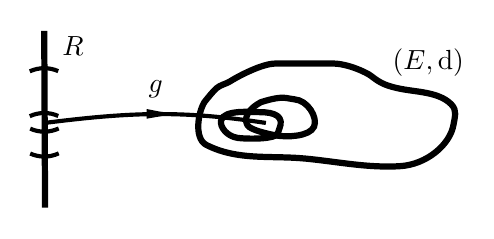
\begin{tikzpicture}[x=0.75pt,y=0.75pt,yscale=-0.6,xscale=0.8]
%uncomment if require: \path (0,300); %set diagram left start at 0, and has height of 300

%Straight Lines [id:da6857889427628007] 
\draw [line width=2.25]    (100,118) -- (100.5,260) ;
%Shape: Arc [id:dp022856158318092845] 
\draw  [draw opacity=0][line width=1.5]  (91.28,150.57) .. controls (94.04,148.9) and (96.97,148) .. (100,148) .. controls (102.93,148) and (105.76,148.84) .. (108.44,150.41) -- (100,208) -- cycle ; \draw  [line width=1.5]  (91.28,150.57) .. controls (94.04,148.9) and (96.97,148) .. (100,148) .. controls (102.93,148) and (105.76,148.84) .. (108.44,150.41) ;  
%Shape: Arc [id:dp8618858057031726] 
\draw  [draw opacity=0][line width=1.5]  (108.72,196.43) .. controls (105.96,198.1) and (103.03,199) .. (100,199) .. controls (97.07,199) and (94.24,198.16) .. (91.56,196.59) -- (100,139) -- cycle ; \draw  [line width=1.5]  (108.72,196.43) .. controls (105.96,198.1) and (103.03,199) .. (100,199) .. controls (97.07,199) and (94.24,198.16) .. (91.56,196.59) ;  
%Shape: Arc [id:dp19616233704048058] 
\draw  [draw opacity=0][line width=1.5]  (108.72,216.43) .. controls (105.96,218.1) and (103.03,219) .. (100,219) .. controls (97.07,219) and (94.24,218.16) .. (91.56,216.59) -- (100,159) -- cycle ; \draw  [line width=1.5]  (108.72,216.43) .. controls (105.96,218.1) and (103.03,219) .. (100,219) .. controls (97.07,219) and (94.24,218.16) .. (91.56,216.59) ;  
%Shape: Arc [id:dp41839281673222306] 
\draw  [draw opacity=0][line width=1.5]  (91.28,186.57) .. controls (94.04,184.9) and (96.97,184) .. (100,184) .. controls (102.93,184) and (105.76,184.84) .. (108.44,186.41) -- (100,244) -- cycle ; \draw  [line width=1.5]  (91.28,186.57) .. controls (94.04,184.9) and (96.97,184) .. (100,184) .. controls (102.93,184) and (105.76,184.84) .. (108.44,186.41) ;  
%Shape: Regular Polygon [id:dp27683657588229815] 
\draw  [line width=2.25]  (272.77,144.33) .. controls (261.5,144.33) and (250.23,144.12) .. (238.96,144.33) .. controls (231.27,144.47) and (217.48,153.96) .. (211.91,158.63) .. controls (209.41,160.73) and (205.86,161.55) .. (203.8,164.08) .. controls (201.21,167.24) and (199.2,170.83) .. (197.03,174.3) .. controls (193.2,180.42) and (189.44,204.16) .. (197.71,209.71) .. controls (216.61,222.41) and (235.93,217.93) .. (257.22,220.61) .. controls (276.7,223.07) and (294.22,228.2) .. (314.02,226.74) .. controls (330.44,225.53) and (344.51,209.23) .. (346.48,193.37) .. controls (347.22,187.45) and (348.9,182.09) .. (345.13,177.02) .. controls (337.39,166.62) and (323.57,167.37) .. (312.67,164.08) .. controls (304,161.46) and (301.35,158.81) .. (296.44,153.86) .. controls (294.23,151.64) and (282.2,143.76) .. (272.77,144.33) -- cycle ;
%Curve Lines [id:da367767170262597] 
\draw [line width=1.5]    (100.25,192) .. controls (153.5,183) and (183.5,182) .. (233.5,192) ;
\draw [shift={(177.27,184.98)}, rotate = 181] [fill={rgb, 255:red, 0; green, 0; blue, 0 }  ][line width=0.08]  [draw opacity=0] (15.6,-3.9) -- (0,0) -- (15.6,3.9) -- cycle    ;
%Shape: Polygon Curved [id:ds9549073342099108] 
\draw  [line width=2.25] [line join = round][line cap = round] (229.83,183.33) .. controls (224.98,183.33) and (208,181.03) .. (206.5,190) .. controls (205.65,195.09) and (209.94,202.74) .. (216.5,204) .. controls (220.72,204.81) and (235.1,205.3) .. (239.5,202) .. controls (240.94,200.92) and (240.93,198.7) .. (241.5,197) .. controls (244.89,186.82) and (239.01,183.33) .. (229.83,183.33) -- cycle ;
%Shape: Regular Polygon [id:dp6827950932437457] 
\draw  [line width=2.25]  (230.5,175.33) .. controls (219.5,183.33) and (221.21,191.42) .. (222.5,194) .. controls (224.38,197.76) and (234.91,200.85) .. (239.5,202) .. controls (245.82,203.58) and (259.8,203.09) .. (262.5,195) .. controls (264.86,187.91) and (258.89,173.7) .. (250.5,173) .. controls (246.13,172.64) and (244.5,169.33) .. (230.5,175.33) -- cycle ;

% Text Node
\draw (109,120.4) node [anchor=north west][inner sep=0.75pt]    {$\mathbb{R}$};
% Text Node
\draw (308,130) node [anchor=north west][inner sep=0.75pt]    {$( E,\mathrm{d})$};
% Text Node
\draw (161,155.4) node [anchor=north west][inner sep=0.75pt]    {$g$};


\end{tikzpicture}
\caption{Example on $\RR$}
    \end{figure}
\end{exampleenv}
\begin{exampleenv}
    Let $(G,\le)$ be a totally ordered set, $\mathcal{F}$ be the ordered topology on $G$. It is generated by $\{G_{>a}\mid a\in G\}\cup\{G_{<b}\mid b\in G\}$. If $l\in G$, then $\mathcal{V}_x(\mathscr{T})$ is generated by 
    $$S_l:=\{G_{>a}\mid a<l\}\cup\{G_{<b}\mid l<b\}.$$
    Assume that $(G,\le)$ is order complete. Let $f:X\longrightarrow G$ be a mapping and $\mathcal{F}$  be  a non-degenerate filter on $X$.
    \newline
    (1) Assume that $f$ converges to $l$ along $\mathcal{F}$. $\forall a< l, \ U_a:=f^{-1}\left(G_{>a}\right)\in \mathcal{F}$. $\forall x\in U_a, f(x)>a$. So $\liminf_{\mathcal{F}}f\ge a$. If $\sup\left(G_{<l}\right)=l$, then $\liminf_{\mathcal{F}}f\ge l.$ If $\sup\left(G_{<l}\right)<l$, we denote $a=\sup\left(G_{<l}\right)$. $\forall a\in U_a, f(x)\ge l$. So $\liminf_{\mathcal{F}}f\ge l$. Similarly, $\liminf_{\mathcal{F}}f\le l$. So $f$ admits $l$ as its limit.
    \newline
    (2) Assume that $\limsup_{\mathcal{F}}f=\liminf_{\mathcal{F}}f=l$. 
    $$\liminf_{\mathcal{F}}f=l\Rightarrow \sup_{U\in \mathcal{F}}f^i(U)=l, \forall a<l, \exists U\in \mathcal{F}, f^i(U)>a, f^{-1}(G_{>a})\in \mathcal{F}.$$
    $$\limsup_{\mathcal{F}}f=l\Rightarrow \forall b>l, f^{-1}(G_{<b})\in \mathcal{F}.$$
    Therefore, $f$ converges to $l$ along $\mathcal{F}$.
\end{exampleenv}


\section{Continuity}
\begin{definitionenv}
    Let $(X,\mathscr{T}_X)$ and $(Y,\mathscr{T}_Y)$ be topological spaces, $f$ be a function from $X$ to $Y$, and $p\in \mathrm{Dom}(f)$. If for any neighborhood $U$ of $f(p)$, there exists a neighborhood $V$ of $p$ such that 
    $$f(V)\subseteq U,$$
    then we say that the function $f$ is \textbf{continuous} at the point $p$. 
    
    If $f$ is continuous at any $p\in \mathrm{Dom}(f)$, then we say that $f$ is \textbf{continuous}.
\end{definitionenv}
\begin{remark}
    \ \newline
    (1) The continuity of $f$ at $p$ is equivalent to:
    $$\underset{x\rightarrow p}{\lim_{x\in \mathrm{Dom}(f)}}f(x)=f(p),$$
    namely, $f$ converges to $f(p)$ when $x$ tends to $p$.
    \newline
    (2) Let $\mathcal{V}_{f(p)}\left(\mathscr{T}_Y\right)$ and $\mathcal{V}_{p}\left(\mathscr{T}_X\right)$ be filters of neighborhoods of $f(p)$ and $p$ respectively. Let $\mathcal{B}_p$ be a filter basis that generates $\mathcal{V}_p\left(\mathscr{T}_X\right)$. Let $S_{f(p)}$ be a subset of $\mathcal{V}_{f(p)}\left(\mathscr{T}_Y\right)$ that generates $\mathcal{V}_{f(p)}\left(\mathscr{T}_Y\right)$. Then the continuity of $f$ at $p$ is equivalent to:
    $$\forall U\in S_{f(p)},\ \exists V\in \mathcal{B}_p,\ f(V)\subseteq U.$$
    In the case where $X$ and $Y$ are metric spaces, this condition becomes:
    $$\forall \varepsilon >0,\ \exists \delta>0,\ \forall x\in \mathrm{Dom}(f),\ \mathrm{d}(x,p)<\delta\Rightarrow \mathrm{d}(f(x),f(p))<\varepsilon.$$
\end{remark}
\begin{propositionenv}
    Let $(X,\mathscr{T}_X),\ (Y,\mathscr{T}_Y),\ (Z,\mathscr{T}_Z)$ be topological spaces. $f: X\longrightarrow Y$, $g: Y\longrightarrow Z$ be functions. $p\in \mathrm{Dom}(g\circ f)$. Assume that $f$ is continuous at $p$ and $g$ is continuous at $f(p)$. Then $g\circ f$ is continuous at $p$.
\end{propositionenv}
\begin{proofenv}
    Let $U$ be a neighborhood of $g\left(f\left(p\right)\right)$. Since $g$ is continuous at $f(p)$, there exists a neighborhood $V$ of $f(p)$ such that $g(V)\subseteq U$. Since $f$ is continuous at $p$, there exists a neighborhood $W$ of $p$, such that $f(W)\subseteq V$. Hence $g\left(f\left(W\right)\right)\subseteq g\left(V\right)\subseteq U.$ So $g\circ f$ is continuous at $p$.
\end{proofenv}
\begin{exampleenv}
    Let $\left(X,\mathscr{T}_X\right)$ be a topological space. Then $\mathrm{Id}_X$ and constant mapping are continuous.
\end{exampleenv}
\begin{theoremenv}
Let $\left(X,\mathscr{T}_X\right)$, $\left(Y,\mathscr{T}_Y\right)$ be topological spaces, $f:X\longrightarrow Y$ a function, $p\in \mathrm{Dom}(f)$. Consider the following conditions:
\newline
(1) $f$ is continuous at $p$.
\newline
(2) For any $(x_n)_{n\in \NN}\in \mathrm{Dom}(f)^{\NN}$, if $\dis \lim_{n\rightarrow \infty}x_n=p$, then 
$$\lim_{n\rightarrow \infty}f(x_n)=f(p).$$
One has (1)$\Rightarrow$(2). If $p$ has a countable basis of neighborhoods, (2)$\Rightarrow$(1).
\end{theoremenv}
\begin{proofenv}
    Let $(x_n)_{n\in\NN}\in \mathrm{Dom}(f)^{\NN}$ such that $\dis \lim_{x\rightarrow \infty}x_n=p$. $f$ is continuous at $p$, so for any neighborhood $U$ of $f(p)$, there exists a neighborhood $V$ of $p$, such that $f(V)\subseteq U$. Since $\dis \lim_{n\rightarrow \infty}x_n=p$, there exists $N\in \NN$, so that for any $n\in \NN_{>N},\ x_n \in V$. Hence for any $n\in \NN_{>N}$, $f(x_n)\in U$. Hence $\dis \lim_{n\rightarrow \infty}f(x_n)=f(p)$.

    Assume that $p$ has a countable basis of neighborhood. Let $(W_n)_{n\in \NN}$ be a sequence of neighborhood of $p$, such that $\{W_n\mid n\in \NN\}$ forms a neighborhood basis. For $n\in \NN$, 
    $$V_n:=\bigcap_{i\in \NN_{\le n}}W_i.$$
    $V_n$ is a neighborhood of $p$. If $f$ is not continuous at $p$, then there exists an neighborhood of $p$, $U$, such that 
    $$\forall n\in \NN,\ f(V_n)\nsubseteq U.$$
    We pick $x_n\in V_n$ but $f(x_n)\notin U.$ For any neighborhood $V$ of $p$, there exists $N\in \NN$ such that $V_N\subseteq V$, so that $x_n\in V$ for any $n\in \NN_{>N}$. Hence, $x_n$ converges to $p$. But $f(x_n)$ cannot converge to $f(p)$.
\end{proofenv}
\begin{lemmaenv}
    Let $(X,\mathscr{T}_X)$ be a topological space. $V\subseteq X$. If $\forall p\in V$, $V$ is a neighborhood of $p$, then $V\in \mathscr{T}_X$. In fact $\forall p\in V$, there exists $W_p\in \mathscr{T}_X$, $p\in W_p\subseteq V$. Hence 
    $$V=\bigcup_{p\in V}\{p\}\subseteq \bigcup_{p\in V} W_p\subseteq V.$$
\end{lemmaenv}
\begin{propositionenv}
    Let $\left(X,\mathscr{T}_X\right)$, $\left(Y,\mathscr{T}_Y\right)$ be topological spaces, $\mathcal{S}\subseteq\mathscr{T}_Y$, $\mathcal{S}$ generates $\mathscr{T}_Y$. The following statements are equivalent:
    \newline
    (1) $f$ is continuous.
    \newline
    (2) For any $U\in \mathscr{T}_Y$, $f^{-1}(U)\in \mathscr{T}_X$.
    \newline
    (3) For any $U\in \mathcal{S}$, $f^{-1}(U)\in \mathscr{T}_X$.
\end{propositionenv}
\begin{proofenv}
    \ \newline
    (1)$\Rightarrow$(2): For any $p\in f^{-1}(U)$, one has $f(p)\in U$. Hence, there is a neighborhood $V_p$ of $p$, $f(V_p)\subseteq U$, or equivalently $V_p\subseteq f^{-1}(U)$. Therefore, $f^{-1}(U)\in \mathscr{T}_X$.
    \newline
    (3)$\Rightarrow$(2): 
    $$\mathscr{T}_{Y}'=\left\{U\in \wp(Y)\mid f^{-1}(U)\in\mathscr{T}_X\right\}$$
    By definition, $\{\varnothing, Y\}\subseteq \mathscr{T}_{Y}'$. If $(U_1,U_2)\in \mathscr{T}_Y'\times\mathscr{T}_Y'$, then $f^{-1}(U_1\cap U_2)=f^{-1}(U_1)\cap f^{-1}(U_2)\in\mathscr{T}_X$. So $U_1\cap U_2\in \mathscr{T}_Y'$. $(U_i)_{i\in I}\in\left(\mathscr{T}_{Y}'\right)^I$, then 
    $$f^{-1}\left(\bigcup_{i\in I}U_i\right)=\bigcup_{i\in I}f^{-1}(U_i)\in \mathscr{T}_X.$$
    So $\mathscr{T}_Y'$ is a topology, by (3), $\mathcal{S}\subseteq \mathscr{T}_Y'\Rightarrow\mathscr{T}_Y\subseteq \mathscr{T}_Y'$.
\end{proofenv}



\section{Initial Topology}
\begin{definitionenv}
    Let $X$ be a set, $\left((Y_i,\mathscr{T}_i)\right)_{i\in I}$ a family of topological spaces, $\left(f_i:X\longrightarrow Y_i\right)_{i\in I}$ a family of mappings. We call \textbf{initial topology} on $X$ induced by $\left(f_i\right)_{i\in I}$ the topology generated by 
    $$\bigcup_{i\in I}\left\{f^{-1}_i(U_i)\mid U_i\in \mathscr{T}_i\right\}.$$
    It is the coarsest topology on $X$ making all $f_i$ continuous.
\end{definitionenv}
\begin{propositionenv}
    Let $\mathscr{T}$ be the initial topology on $X$ induced by $\left(f_i\right)_{i\in I}$. 
    \newline
    (1) $$\mathcal{B}= \left\{ \bigcap_{j\in J}f^{-1}_j(U_j)\mid J\subseteq I \text{ finite, }\left(U_j\right)_{j\in J}\in \prod_{j\in J}\mathscr{T}_j\right\}$$
    is topological basis that generates $\mathscr{T}$.
    \newline
    (2) Let $(Z,\mathscr{T}_Z)$ be topological space, $h:Z\longrightarrow X$ be a function and $p\in \mathrm{Dom}(f)$. Then $h$ is continuous at $p$ if and only if $\forall i\in I,\ f_i\circ h$ is continuous at $p$.
\end{propositionenv}
\begin{proofenv}
    \ \newline
    (1) Let 
    $$S=\bigcup_{i\in I}\left\{f^{-1}_{i}\left(U_i\right)\mid U_i\in \mathscr{T}_i\right\},$$
    $\mathcal{B}'$ be the set of the intersections of all finitely elements of $S$ (We have proved that $\mathcal{B}'$ is a basis of $\mathscr{T}$). $\mathcal{B}\subseteq\mathcal{B}'$. Let $i_1,\dots, i_n$ elements of $I$, $U_{i_k}\in \mathscr{T}_{i_k}$, $J=\{i_1,\dots,i_n\},\ j\in J$, $A_j=\left\{k\in\{1,\dots,n\}\mid i_k=j\right\}$, $\dis W_j=\bigcap_{k\in A_j}U_{i_k}$.
    $$\bigcap_{k=1}^{n}f^{-1}_{i_k}\left(U_{i_k}\right)=\bigcap_{j\in J}f^{-1}_{j}\left(W_j\right)\in \mathcal{B}.$$
    (2) Since $f_i$ is continuous at $p$, if $h$ is continuous then $\forall i\in I$, $f_i\circ h$ is continuous. Assume $\forall i\in I,\ f_i\circ h$ is continuous, then 
    $$\forall i\in I,\ \forall U_i\in \mathscr{T}_i,\ \left(f_i\circ h\right)^{-1}\left(U_i\right)=h^{-1}\left(f_i^{-1}\left(U_i\right)\right).$$
    Therefore, for any $V\in S$, $h^{-1}(V)\in \mathscr{T}_Z.$ Hence $h$ is continuous.
\end{proofenv}
\begin{exampleenv}
    Let $(X_i,\mathscr{T}_i)$ be topological spaces, $X=\prod_{i\in I}X_i$, $\pi_i:X\longrightarrow X_i$ be a projection. The initial topology on $X$ induced by $(\pi_i)_{i\in I}$ is called the \textbf{product topology}.
\end{exampleenv}



\section{Uniform Continuity}
\begin{definitionenv}
    Let $(X, \mathrm{d}_X),\ (Y,\mathrm{d}_Y)$ be semimetric spaces, $f:X\longrightarrow Y$ be a function, $\alpha \in \RR_{\ge0}$. If for any $(x_1,x_2)\in \mathrm{Dom}(f)^2$, $\mathrm{d}\left(f(x_1),f(x_2)\right)\le \alpha\cdot \mathrm{d}(x_1,x_2)$, then we say that $f$ is $\alpha$-Lipschitzian. If there exists $\alpha\in \RR_{\ge 0}$ such that $f$ is \textbf{$\alpha$-Lipschitzian}, then we say that $f$ is \textbf{Lipschitzian}. 

    If 
    $$\forall \varepsilon>0,\exists \delta>0,\ \forall (x_1,x_2)\in \mathrm{Dom}(f)^2,\ \mathrm{d}_X(x_1,x_2)<\delta\Rightarrow \mathrm{d}(f(x_1),f(x_2))<\varepsilon,$$
    then we say that $f$ is \textbf{uniformly continuous}.
\end{definitionenv}
\begin{propositionenv}
    Let $(X,\mathrm{d}_X),\ (Y,\mathrm{d}_Y)$ be semimetric spaces, $f:X\longrightarrow Y$ be a function. If $f$ is uniformly continuous, then $f$ continuous.
\end{propositionenv}
\begin{proofenv}
Let $p\in \mathrm{Dom}(f)$. For $\varepsilon>0$, there exists $\delta>0$ such that 
$$\forall (x_1,x_2)\in \mathrm{Dom}(f)^2,\ \mathrm{d}_X(x_1,x_2)<\delta\Rightarrow \mathrm{d}(f(x_1),f(x_2))<\varepsilon.$$
In particular, 
$$\forall x\in \mathrm{Dom}(f),\ \exists \delta>0,\ \mathrm{d}_X(x,p)<\delta\Rightarrow \mathrm{d}_Y(f(x),f(p))<\varepsilon.$$
\end{proofenv}
\begin{definitionenv}
    Let $K$ be a field, we call absolute value on $K$ any mapping,
    $$\left|\ \cdot\ \right|: K\longrightarrow \RR_{\ge 0},$$
    (1) $\forall a\in K,\ a=0_K$ if and only if $\left|a\right|=0.$
    \newline
    (2) $\forall (a,b)\in K\times K,\ \left|ab\right|=\left|a\right|\left|b\right|.$
    \newline
    (3) $\forall (a,b)\in K\times K,\ \left|a+b\right|\le \left|a\right|+\left|b\right|.$
    \newline
    The pair $(K,\left|\ \cdot\ \right|)$ is called a \textbf{valued field}.

\end{definitionenv}
\begin{exampleenv}
    Let $(K,\le)$ be a totally ordered field, then $\left|a\right|=\max\{-a,a\}$ is an absolute value on $K$.
\end{exampleenv}
\begin{exampleenv}
    Let $p$ be a prime number. Any non-zero rational number $\alpha$ can be written in the form
    $$\alpha=p^{\mathrm{ord}_p(\alpha)}\cdot\frac{m}{n},$$
    where, $\mathrm{ord}_p(\alpha)\in \ZZ,\ p\nmid mn$. If $\alpha=0$, we set (by convention) $\mathrm{ord}_p(\alpha)=+\infty.$

    \textbf{Properties:} 
    \newline
    (1) $\mathrm{ord}_p(\alpha\beta)=\mathrm{ord}_p(\alpha)+\mathrm{ord}_p(\beta)$.
    \newline
    (2) $\alpha=p^{\mathrm{ord}_p(\alpha)}\frac{m}{n},\ \beta=p^{\mathrm{ord}_p(\beta)}\frac{u}{v}$, $\mathrm{ord}_p(\alpha)>\mathrm{ord}_p(\beta)$, $p\nmid nvu$.
    $$\alpha+\beta=p^{\mathrm{ord}_p(\beta)}\frac{p^{\mathrm{ord}(\alpha)-\mathrm{ord}(\beta)}mv+nu}{nv}.$$
    (3) If $\mathrm{ord}(\alpha)=\mathrm{ord}(\beta)$, then $\mathrm{ord}_{p}(\alpha+\beta)\ge \mathrm{ord}_p(\alpha)=\mathrm{ord}_p(\beta).$
    $$\alpha+\beta=p^{\mathrm{ord}_p(\alpha)}\frac{mv+nu}{nv}.$$
\end{exampleenv}
\begin{propositionenv}
    The mapping 
    $$\left|\ \cdot\ \right|_{p}: \QQ\longrightarrow \RR_{\ge 0},$$
    $$\left\{\begin{matrix}
        &|\alpha|_p=p^{-\mathrm{ord}(\alpha)}, &\text{if } \alpha\neq0\\
        &|\alpha|_p=0, &\text{if } \alpha=0
    \end{matrix}\right.$$
    is an absolute value on $\QQ$.
\end{propositionenv}
\begin{proofenv}
    If $\alpha=0$, then $|\alpha|_p>0$. If $(\alpha,\beta)\in \QQ^2$, when $0\in \{\alpha,\beta\}$, then $\alpha\beta=0$ and $0=|\alpha\beta|_p=|\alpha|_p|\beta|_p$. When $0\notin\{\alpha,\beta\}$, 
    $$|\alpha\beta|_p=p^{-\mathrm{ord}_p(\alpha\beta)}=p^{-\mathrm{ord}_p(\alpha)-\mathrm{ord}_p(\beta)}= |\alpha|_p|\beta|_p.$$
    If $\alpha=0$, $|\alpha\beta|_p= |\beta|_p.$ If $\beta=0$, $|\alpha\beta|_p= |\alpha|_p.$, if $0\notin\{\alpha,\beta\}$,
    $$|\alpha+\beta|_p=p^{-\mathrm{ord}_p(\alpha+\beta)}\le p^{\max\{\mathrm{ord}_p(\alpha),\mathrm{ord}_p(\beta)\}}\le \max\{|\alpha|_p,|\beta|_p\}\le |\alpha|_p+|\beta|_p.$$
\end{proofenv}
\begin{remark}
    Let $(K,\left|\ \cdot\ \right|)$ be a valued field. If for any $(\alpha,\beta)\in K^2$ satisfies $|\alpha+\beta|\le \max\{|\alpha|,|\beta|\}$, we say that $(K,\left|\ \cdot\ \right|)$ is \textbf{non-archimedean}, otherwise, we say that $(K,\left|\ \cdot\ \right|)$ is \textbf{archimedean}. $(\RR,\left|\ \cdot\ \right|)$ and $(\QQ,\left|\ \cdot\ \right|)$ are archimedean.
\end{remark}
\begin{definitionenv}
    Let $(K,\left|\ \cdot \ \right|)$ be a valued filed, $V$ a vector spaced over $K$. We call \textbf{seminorm} on $V$ any mapping 
    $$|\!| \cdot |\!|:V\longrightarrow \RR_{\geq 0}$$ 
    that satisfies the following conditions:
    \newline
    (1) $\forall (a,x)\in K\times V,\ |\!|ax|\!|=|a|\cdot|\!|x|\!|$.
    \newline
    (2) $\forall (x,y)\in V\times V,\ |\!|x+y|\!|\le |\!|x|\!|+|\!|y|\!|.$
    \newline
    Note that (1) implies that $|\!|0_V|\!|=|0_K|\cdot|\!|0_V|\!|=0$.

    The pair $(V,|\!| \cdot |\!|)$ is called \textbf{seminormed vector space} \textit{over} $(K,\left|\ \cdot\ \right|)$. If $\forall(x,y)\in V\times V,\ |\!|x+y|\!|\le \max\{|\!|x|\!|,|\!|y|\!|\}$, then we say that $|\!|\cdot|\!|$ is \textbf{ultrametric}. If $\forall x\in V\backslash\{0\}$, $|\!|x|\!|>0$, then we say that $|\!| \cdot|\!|$ is a \textbf{norm} and $(V,|\!| \cdot |\!|)$ is a \textbf{normed vector space} \textit{over} $(K,\left|\ \cdot\ \right|)$.
\end{definitionenv}
\begin{exampleenv}
    $\mathrm{d}:V\times V\longrightarrow \RR_{\ge 0}$, $\mathrm{d}(x,y):=|\!|x-y|\!|$ is a semi-metric. 
\end{exampleenv}
\begin{exampleenv}
    Let $(K,\left|\ \cdot\ \right|)$ be a valued field.
    \newline
    (1) $(K,\left|\ \cdot\ \right|)$ is a normed vector space over $(K,\left|\ \cdot\ \right|)$. ($\mathrm{d}(x,y)=|x-y|$ is a metric.)
    \newline
    (2) Let $(V_1,|\!|\cdot|\!|_1),\dots, (V_n,|\!|\cdot|\!|_n)$ be seminormed vector spaces over $(K,\left|\ \cdot\ \right|)$, $V=V_1\oplus\dots\oplus V_n$.
    $$|\!|\cdot|\!|_{l^\infty}:V\longrightarrow \RR_{\ge0},\ (x_1,\dots,x_n)\longmapsto\max_{i\in\{1,\dots,n\}}|\!|x_i|\!|_{i},\ x_i\in V_i,\ i\in \{1,\dots,n\},$$
    $$|\!|\cdot|\!|_{l^1}:V\longrightarrow \RR_{\ge0},\ (x_1,\dots,x_n)\longmapsto\sum_{i\in\{1,\dots,n\}}|\!|x_i|\!|_{i},\ x_i\in V_i,\ i\in \{1,\dots,n\}.$$
    $\forall \lambda\in K, \ \forall (x_1,\dots,x_n)\in V,$ 
    \begin{align*}
        \pl \lambda(x_1,\dots,x_n)\pl_{l^\infty}&=\pl(\lambda\cdot x_1,\dots,\lambda x_n)\pl_{l^\infty}\\
        &=\max_{i\in\{1,\dots,n\}}\pl\lambda x_i\pl_i\\
        &=\max_{i\in\{1,\dots,n\}}\left|\lambda\right||\!| x_i|\!|_{i}\\
        &=|\lambda|\max_{i\in\{1,\dots,n\}}|\!|x_i|\!|_{i}\\
        &=|\lambda|\cdot |\!|(x_1,\dots,x_n)|\!|_{l^\infty}.
    \end{align*}
    \begin{align*}
        \pl \lambda(x_1,\dots,x_n)\pl_{l^1}&=\pl(\lambda\cdot x_1,\dots,\lambda x_n)\pl_{l^1}\\
        &=\sum_{i\in\{1,\dots,n\}}\pl\lambda x_i\pl_i\\
        &=\sum_{i\in\{1,\dots,n\}}\left|\lambda\right||\!| x_i|\!|_{i}\\
        &=|\lambda|\sum_{i\in\{1,\dots,n\}}|\!|x_i|\!|_{i}\\
        &=|\lambda|\cdot |\!|(x_1,\dots,x_n)|\!|_{l^1}.
    \end{align*}
    $\forall x=(x_1,\dots,x_n),\ y=(y_1,\dots,y_n)\in V$,
    \begin{align*}
        \pl x+y\pl_{l^\infty}&=\pl(x_1+y_1,\dots,x_n+y_n)\pl_{l^\infty}=\max_{i\in\{1,\dots,n\}}\pl x_i+y_i\pl_i\\
        &\le \max_{i\in\{1,\dots,n\}}\pl x_i\pl_i+\pl y_i\pl_i\le \pl x\pl_{l^\infty}+\pl y\pl_{l^\infty}.
    \end{align*}
    \begin{align*}
        \pl x+y\pl_{l^1}&=\sum_{i\in\{1,\ldots,n\}}\pl x_i+y_i\pl_i\\
        &\le \sum_{i\in\{1,\dots,n\}}\pl x_i\pl_i+\pl y_i\pl_i= \pl x\pl_{l^1}+\pl y\pl_{l^1}.
    \end{align*}
    (3) Let $(V,\pl\cdot\pl)$ be a seminormed vector space over $K$, $f:W\longrightarrow V$ be a $K$-linear mapping. We denote by $\pl\cdot\pl_f$ the mapping $W\longrightarrow \RR_{\ge 0}$ define as 
    $$\forall x\in W, \ \pl x\pl_f:=\pl f(x)\pl.$$
    $\forall (\lambda,x)\in K\times W$, 
    $$\pl \lambda x\pl_f=\pl f(\lambda x)\pl =\pl \lambda f(x)\pl =\left|\lambda\right|\cdot\pl f(x)\pl=\lambda \pl x\pl_f.$$
    $\forall (x,y)\in W\times W$, 
    $$\pl x+y\pl_f=\pl f(x+y)\pl=\pl f(x)\pl+\pl f(y)\pl\le \pl x\pl_f+\pl y\pl_f.$$
    Therefore, $\pl\cdot\pl_f$ is a seminorm on $W$, called the \textbf{seminorm} \textit{induced by (the $K$-linear) mapping $f$}.
    \newline
    (4) Let $(V,\left|\ \cdot\ \right|)$ be a seminormed vector space over $K$, let $\pi:V\longrightarrow E$ be a surjective $K$-linear mapping. We denote by $\pl\cdot\pl_\pi$ the mapping
    $$E\longrightarrow \RR_{\ge 0},$$
    $$\alpha\longmapsto \inf_{x\in \pi^{-1}(\alpha)}\pl x\pl.$$
    If $(\lambda,\alpha)\in K\times E$,
    $$\pl \lambda\alpha\pl_\pi=\inf_{x\in \pi^{-1}(\lambda\alpha)}\pl x \pl=\inf_{x\in \pi^{-1}(\alpha)}\left|\lambda\right|\pl x\pl=\left|\lambda\right|\pl\alpha\pl_\pi.$$
    If $(\alpha,\beta)\in E\times E,$
    \begin{align*}
         \pl\alpha+\beta\pl_\pi=\inf_{z\in\pi^{-1}(\alpha+\beta)}\pl z\pl &=\inf_{(x,y)\in \pi^{-1}(\alpha)\times\pi^{-1}(\beta)}\pl x+y\pl \\
         &\le\inf_{(x,y)\in \pi^{-1}(\alpha)\times\pi^{-1}(\beta)}\pl x\pl +\pl y\pl\\
         &=\inf_{x\in \pi^{-1}(\alpha)}\pl x\pl+\inf_{y\in \pi^{-1}(\beta)}\pl y\pl.
    \end{align*}
    Hence $\pl\cdot\pl_\pi$ is a seminorm on $E$ called the \textbf{quotient seminorm} \textit{of $\pl\cdot\pl$ induced by $\pi$.} 
\end{exampleenv}
\begin{propositionenv}
    Let $(V,\pl\cdot\pl)$ be a seminormed vector space over a valued field $(K,\left|\ \cdot\ \right|)$.
    \newline
    (1) For any $a\in V$, the mapping $\tau_a:V\longrightarrow V,\ \tau_a(x)=x+a$ is $1$-Lipschitzian.
    \newline
    (2) For any $\lambda\in K$, the mapping $m_\lambda:V\longrightarrow V,\ m_\lambda(x):=\lambda\cdot x$ is $\lambda$-Lipschitzian.
    \newline
    (3) The mapping $\pl\cdot\pl: V\longrightarrow \RR$ is $1$-Lipschitzian.
\end{propositionenv}
\begin{proofenv}
    \ \newline
    (1) $\forall(x,y)\in V\times V,\ \pl \tau_a(x)-\tau_a(y)\pl=\pl(x+a)-(y+a)\pl=\pl x-y\pl$.
    \newline
    (2) $\forall (x,y)\in V\times V,\ \pl m_\lambda(x)-m_\lambda(y)\pl=\pl\lambda x-\lambda y\pl=\left|\lambda\right|\pl x-y\pl $.
    \newline
    (3) $\forall (x,y)\in V\times V,\ \pl x\pl =\pl (x-y)+y\pl\le\pl y\pl+\pl x-y\pl$. So $\pl x\pl -\pl y\pl \le \pl x-y\pl.$ Similarly, $\pl y\pl -\pl x\pl \le \pl y-x\pl.$ Hence,
    $$\left|\pl x\pl-\pl y\pl\right|\le \pl x-y\pl.$$
\end{proofenv}
\begin{definitionenv}
    $(E,\pl\cdot\pl_E),(F,\pl\cdot\pl_F)$ be two seminormed vector spaces over a valued field $(K,\left|\ \cdot\ \right|)$, and $\varphi$ a $K$-linear mapping from $E$ to $F$. We define $\pl\varphi\pl\in \left[0,+\infty\right]$  as
    $$\pl\varphi\pl:=\sup_{\substack{x\in E\\ \pl x\pl_E\neq 0}}\frac{\pl\varphi(x)\pl_F}{\pl x\pl_E}.$$
    In the case where $\pl x\pl_E=0$, for any $x\in E$, by convention, $\pl\varphi(x)\pl$ is defined to be $0$. If $\pl \varphi\pl<+\infty$, we say that $\varphi$ is bounded. We denote by $\mathscr{L}(E,F)$ the set of all bounded $K$-linear mappings from $E$ to $F$.
\end{definitionenv}
\begin{remark}
    In the case when $(E,\pl \cdot\pl_E)=(K,\pl\cdot\pl) $, 
    $$\pl\varphi\pl=\sup_{x\in\mathcal{B}(0,1)}\pl\varphi(x)\pl_{F}.$$
\end{remark}
\begin{propositionenv}
    \ \newline
    (1) For any $\varphi\in\mathscr{L}(E,F)$ be the mapping $\varphi$ is $\pl\varphi\pl$-Lipschitzian. In particular, $\varphi$ is continuous.
    \newline
    (2) Suppose that there exists $\lambda\in K$, such that $|\lambda|>1$. If $\varphi: E\longrightarrow F$  is continuous at $0_E$, then $\varphi\in \mathscr{L}(E,F)$.
\end{propositionenv}
\begin{proofenv}
    For any $(x,y)\in E\times E$:
    \newline
    (1) $\pl\varphi(x)-\varphi(y)\pl_{F}=\pl\varphi(x-y)\pl_{F}\le \pl\varphi\pl\pl x-y\pl_{E}$.
    \newline
    (2) $\mathcal{B}(0_F,1):=\{\alpha\in F\mid \pl\alpha\pl_{F}<1\}$ is a neighborhood of $0_F$. There exists $\varepsilon>0$ such that 
    $$\varphi(\overline{\mathcal{B}}(0_E,\varepsilon))\subseteq\mathcal{B}(0_F,1)$$
    where $$\overline{\mathcal{B}}(0_E,\varepsilon):=\{x \in E\mid \pl x\pl_E<\varepsilon\}.$$
    Let $x\in E\backslash \{0\}$, there exists $n\in \ZZ$, such that $\pl\lambda ^n x\pl_E=\left|\lambda\right|^n\pl x\pl_E<\varepsilon$ and $\pl \lambda^{n+1}x\pl_{E}=\left|\lambda\right|^{n+1}\pl x\pl_E\ge \varepsilon$. Thus,
    $$\pl \varphi(x)\pl_F=\pl \lambda^{-n}\varphi(\lambda^n x)\pl_{F}=\left|\lambda\right|^{-n}\pl \varphi(\lambda^n x)\pl_{F}\le \left|\lambda\right|^{-n}\le\frac{\left|\lambda\right|}{\varepsilon}\pl x\pl_E.$$
    Therefore, $\pl\varphi\pl\le \frac{\lambda}{\varepsilon}$.
\end{proofenv}
\begin{propositionenv}
    Let $(E,\pl\cdot\pl_E),(F,\pl\cdot\pl_F)$ be two seminormed vector spaces over a valued field $(K,\left|\ \cdot\ \right|)$. Then $\mathscr{L}(E,F)$ is a vector subspace of $F^E$, and $\pl\cdot\pl$ is a seminorm on $\mathscr{L}(E,F)$, called the operator seminorm.
\end{propositionenv}
\begin{proofenv}
    Let $\varphi,\psi$ be to $K$-linear mappings from $E$ to $F$. For any $x\in E$, such that $\pl x\pl_E\neq0$.
    \begin{align*}
        \pl(\varphi+\psi)(x)\pl_F=&\pl\varphi(x)+\pl\psi(x)\pl_F\le \pl\varphi(x)\pl_F+\pl\psi(x)\pl_F\\
        \le& \pl\varphi\pl\pl x\pl_E+\pl\psi\pl\pl x\pl_E=\left(\pl\varphi\pl+\pl\psi\pl\right)\pl x\pl_E.
    \end{align*}
    $$\pl\varphi+\psi\pl\le\pl\varphi\pl+\pl\psi\pl.$$
    So, $\varphi,\psi\in \mathscr{L}(E,F)\Rightarrow \varphi+\psi\in \mathscr{L}(E,F)$.
    Let $\lambda\in K^\times$ and $\varphi\in \mathscr{L}(E,F)$, for any $x\in E$, $\pl x\pl _E\neq0$. One has 
    $$\pl (\lambda\varphi)(x)\pl_{F}=\pl\lambda\cdot\varphi(x)\pl_F=\left|\lambda\right|\pl\varphi(x)\pl_F \le \left|\lambda\right|\pl\varphi\pl\pl x\pl_E.$$
    So, $\pl\lambda\pl\le\left|\lambda\right|\pl\varphi\pl$, $\lambda\varphi\in \mathscr{L}(E,F)$. So $\mathscr{L}(E,F)$ is a vector subspace of $F^E$. Note that we can apply to $\lambda^{-1}$ and $\lambda\varphi$ and get 
    $$\pl \lambda^{-1}\cdot\lambda\varphi\pl=\pl\varphi\pl\le \left|\lambda^{-1}\right|\pl\lambda\varphi\pl=\left|\lambda\right|^{-1}\pl\lambda\varphi\pl,\ \left|\lambda\right|\le\pl\lambda\varphi\pl.$$
    Hence, $\left|\lambda\right|\pl\varphi\pl=\pl\lambda\varphi\pl$ and therefore $\pl\cdot\pl$ is a seminorm on $\mathscr{L}(E,F)$.
\end{proofenv}
\begin{definitionenv}
    Let $E$ be a vector space over $K$, and $\pl\cdot\pl_1$ and $\pl\cdot\pl_2$  be seminorms on $E$. We say that $\pl\cdot\pl_1$ and $\pl\cdot\pl_2$ are equivalent, if there exists $c_1, c_2\in \RR_{>0}$ such that 
    $$\forall x\in E,\ c_1\pl x\pl_1\le\pl x\pl_2\le c_2\pl x\pl_1.$$
\end{definitionenv}
\begin{propositionenv}
    Let $E$ be a vector space over $K$, and $\pl\cdot\pl_1$ and $\pl\cdot\pl_2$  be seminorms on $E$. If $\pl\cdot\pl_1$ and $\pl\cdot\pl_2$ are equivalent, then they define the same topology on $E$.
\end{propositionenv}
\begin{proofenv}
    Let $\mathscr{T}_1$ and $\mathscr{T}_2$ to be the topologies defined by $\pl\cdot\pl_1$ and $\pl\cdot\pl_2$, respectively. Then 
    $$\mathrm{Id}_E:(E,\mathscr{T}_1)\longrightarrow(E,\mathscr{T}_2)$$
    is bounded. So it is continuous, so $\mathscr{T}_2\subseteq\mathscr{T}_1$. Similarly, $\mathscr{T}_1\subseteq\mathscr{T}_2$.
\end{proofenv}
\begin{propositionenv}
    Let $n\in\NN_{\ge 1}$, and $(X_i,\mathrm{d}_i),\ i\in\{1,2,\ldots,n\}$ be $n$ seminormed vector spaces over $K$. Let $\dis X=\prod_{i=1}^nX_i$ and
    $$\mathrm{d}:X\times X\longrightarrow \RR_{\ge 0},$$
    $$\mathrm{d\left((x_1,\ldots,x_n),(y_1,\ldots,y_n)\right)}\longmapsto \max_{i\in\{1,\ldots,n\}}\mathrm{d}_i(x_i,y_i).$$
    Then $\mathrm{d}$ is a semimetric on $X$, and the topology  induced by $\mathrm{d}$ is the product topology of $\mathscr{T}_{\mathrm{d}_i}$ (topology induced on $X_i$ by $\mathrm{d}_i$) $i\in\{1,\dots,n\}$.

\end{propositionenv}
\begin{proofenv}
    \ \newline
    (1) $\mathrm{d}\left((x_1,\dots,x_n),(x_1,\dots,x_n)\right)=\max_{i\in\{1,\dots,n\}}\mathrm{d}_i(x_i,x_i)=0$.
    \newline
    (2) \begin{align*}
        &\mathrm{d}\left((x_1,\dots,x_n),(y_1,\dots,y_n)\right)=\max_{i\in\{1,\dots,n\}}\mathrm{d}_i(x_i,y_i)\\
        =&\max_{i\in\{1,\dots,n\}}\mathrm{d}_i(y_i,x_i)=\mathrm{d}\left((y_1,\dots,y_n),(x_1,\dots,x_n)\right).
    \end{align*}
    (3) \begin{align*}
        &\mathrm{d}((x_1,\dots,x_n),(z_1,\dots,z_n))\\
        =&\max_{i\in\{1,\dots,n\}}\mathrm{d}_i(x_i,z_i)\\
        \le&\max_{i\in\{1,\dots,n\}}\mathrm{d}_i(x_i,y_i)+\max_{i\in\{1,\dots,n\}}\mathrm{d}_i(y_i,z_i)\\
        =&\mathrm{d}((x_1,\dots,x_n),(y_1,\dots,y_n))+\mathrm{d}((y_1,\dots,y_n),(z_1,\dots,z_n)).
    \end{align*}
    So $\mathrm{d}$ is a semimetric on $X$. For $i\in \{1,\dots,n\}$, $\mathscr{T}_i:=\mathscr{T}_{\mathrm{d}_i}$, where $\mathscr{T}_\mathrm{d}$ is the topology induced by $\mathrm{d}$. Let $\pi_i: X\longrightarrow X_i$ be the project mapping (continuous with the product topology on $X$.) For any $x=(x_1,\dots,x_n), y=(y_1,\dots,y_n)$ in $X$,
    $$\mathrm{d}(x,y)=\max_{i\in\{1,\dots,n\}}\mathrm{d}_i(x_i,y_i)=\max_{i\in\{1,\dots,n\}}\mathrm{d}_i(\pi_i(x),\pi_i(y)),$$
    have $\forall i\in\{1,\dots,n\}$, $\mathrm{d}_i(x_i,y_i)\le \mathrm{d}(x,y)$ 
    which implies that 
    $$\mathrm{Id}_X:(X,\mathscr{T}_\mathrm{d})\longrightarrow (X,\mathscr{T})$$
    is continuous. So $\mathscr{T}\subseteq\mathscr{T}_\mathrm{d}.$
    \begin{align*}
        \mathcal{B}((p_1,\dots,p_n),\varepsilon)=&\{(x_1,\dots,x_n)\mid \mathrm{d}((p_1,\dots,p_n),(x_1,\dots,x_n))<\varepsilon\}\\
        =&\prod_{i=1}^n\mathcal{B}(p_i,\varepsilon)\in\mathscr{T}.
    \end{align*}
\end{proofenv}



\section{Closed Subsets}
\begin{exampleenv}[Review of open subsets]
    In $\RR$, an interval of the form $\interval[open]{a}{b}$ is open, since $\interval[open]{a}{b}=\mathcal{B}(\frac{a+b}{2},\frac{b-a}{2})$. An interval of the form $\interval[open]{a}{+\infty}$ is open, since $\dis \interval[open]{a}{+\infty}=\bigcup_{n\in\NN_{\ge 1}}\interval[open]{a}{a+n}$.
\end{exampleenv}
\begin{definitionenv}
    Let $(X,\mathscr{T})$ be a topological space. We say a subset $Y$ of $X$ is \textbf{closed} if $X\setminus Y$ is open.
\end{definitionenv}
\begin{remark}
    \ \newline
    (1) $\varnothing$, $X$ are closed.
    \newline
    (2) If $F_1$, $F_2$ are closed subset of $X$, then $F_1\cup F_2$ is closed.
    \newline
    (3) If $(F_i)_{i\in I}$ is a non-empty family of closed subsets of $X$, then $\dis \bigcap_{i\in I}F_i$ is closed.
\end{remark}
\begin{exampleenv}
    Let $(a,b)\in \RR^2$, $a<b$, then $[a,b]\subseteq \RR^2$ is closed. Moreover, $\interval[open left]{-\infty}{a}$ is closed.
\end{exampleenv}
\begin{propositionenv}
    Let $(X,\mathscr{T}_X)$ and $(Y,\mathscr{T}_Y)$ be topological spaces, and $f:X\longrightarrow Y$ be a mapping, then the following statements are equivalent:
    \newline
    (1) $f$ is continuous.
    \newline
    (2) For any closed subset $F$ of $Y$, $f^{-1}(F)$ is a closed subset of $X$.
\end{propositionenv}
\begin{proofenv}
    \ \newline
    (1) $\Leftrightarrow$ (2): $f$ is continuous if and only if, for any open subset $U$ of $Y$, $f^{-1}(U)\in \mathscr{T}_X$. Let $F\subseteq Y$ be closed, then $Y\backslash F$ is open. So
    $f^{-1}(Y\backslash F)=X\backslash f^{-1}(F)$ is open, so $f^{-1}(F)$ is closed.
    \newline
    (2) $\Leftrightarrow$ (1): Let $U\in \mathscr{T}_Y$, then $F=Y\backslash U$ is closed, so $f^{-1}(F)=X\backslash f^{-1}(U)$ is closed. So $f^{-1}(U)\in \mathscr{T}_Y$.
\end{proofenv}
\begin{exampleenv}
    \ \newline
    In $\RR^2$, $\{(x,y)\in \RR^2\mid x\ge 1\}$ is closed. Since $\RR^2\backslash\{(x,y)\mid x\ge 1\}=\interval[open]{-\infty}{0}\times \RR$. Since $f(x,y)=x+y$ is continuous, then $f^{-1}(\interval[open right]{0}{+\infty})=\{(x,y)\in \RR^2\mid x+y\ge 0\}$ is closed.
\end{exampleenv}
\begin{exampleenv}
    Let $(X,\mathrm{d})$ be a semimetric space. Let $Y\subseteq X$, $Y\neq\varnothing$. We define, for any $x\in X$,
    $$\mathrm{d}(x,Y)=\inf_{y\in Y}\mathrm{d}(x,y)\in \RR_{\ge 0}.$$
\begin{figure}[H]
    
\begin{center}
        

\tikzset{every picture/.style={line width=0.75pt}} %set default line width to 0.75pt        

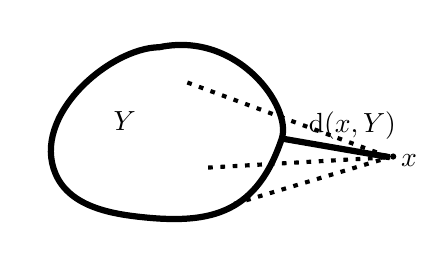
\begin{tikzpicture}[x=0.75pt,y=0.75pt,yscale=-1,xscale=1]
%uncomment if require: \path (0,300); %set diagram left start at 0, and has height of 300

%Shape: Polygon Curved [id:ds27882773645222514] 
\draw  [line width=2.25] [line join = round][line cap = round] (219.5,106) .. controls (195.45,106.4) and (157.57,139.15) .. (169.5,167) .. controls (176.48,183.3) and (197.45,186.5) .. (212.5,188) .. controls (244.94,191.24) and (266.64,185.58) .. (278.5,150) .. controls (283.51,134.98) and (257.5,98.09) .. (219.5,106) -- cycle ;
%Shape: Free Drawing [id:dp255407836209968] 
\draw  [line width=2.25] [line join = round][line cap = round] (332.17,158.67) .. controls (332.17,158.67) and (332.17,158.67) .. (332.17,158.67) ;
%Straight Lines [id:da009494640139930732] 
\draw [line width=2.25]    (278.5,150) -- (330.5,159) ;
%Straight Lines [id:da3200364645577044] 
\draw [line width=1.5]  [dash pattern={on 1.69pt off 2.76pt}]  (255.64,181.46) -- (330.5,159) ;
%Straight Lines [id:da7022259042728503] 
\draw [line width=1.5]  [dash pattern={on 1.69pt off 2.76pt}]  (233,123) -- (330.5,159) ;
%Straight Lines [id:da6184331447803212] 
\draw [line width=1.5]  [dash pattern={on 1.69pt off 2.76pt}]  (243,164) -- (330.5,159) ;

% Text Node
\draw (290,135.4) node [anchor=north west][inner sep=0.75pt]    {$\mathrm{d}( x,Y)$};
% Text Node
\draw (334.5,156.4) node [anchor=north west][inner sep=0.75pt]    {$x$};
% Text Node
\draw (196,135.4) node [anchor=north west][inner sep=0.75pt]    {$Y$};


\end{tikzpicture}
    \end{center}
    \caption{Definition of $\dd(\cdot, Y)$.}
\end{figure}
    The mapping $\dd(\cdot,Y): X\longrightarrow \RR$, $x\longmapsto \mathrm{d}(x,Y)$ is $1$-Lipschitzian.
    \newline
    Let $(x,x')\in X\times X$, $\forall y\in Y$,
    $$\dd (x,Y)-\dd(x',y)\le \dd(x,y)-\dd(x',y)\le\dd(x,x').$$
    Taking the supremum, we get 
    $$\dd(x,Y)-\dd(x',Y)\le \dd(x,x').$$
    By symmetry between $x$ and $x'$, $\dd(x',Y)-\dd(x,Y)\le \dd(x,x')$. So 
    $$|\dd(x,Y)-\dd(x',Y)|\le |\dd(x,x')|.$$
    For any $r>0$, define 
    $$B(Y,r):=\{x\in X\mid \dd(x,Y)< r\},$$
    $$\overline{B}(Y,r):=\{x\in X\mid \dd(x,Y)\le r\}$$
    $B(Y,r)$ is open, $\overline{B}(Y,r)$ is closed. If $Y=\{y\}$ is a one point set, $B(Y,r)$ and $\overline{B}(Y,r)$ are defined as $B(y,r)$ and $\overline{B}(y,r)$ respectively.
\end{exampleenv}
\begin{definitionenv}
    Let $(X,\mathscr{T})$ be a topological space. 
    \newline
    (1) Let $\mathcal{F}$ be a non-degenerate filter, an element $p\in X$ is called \textbf{adherent point} \textit{of} $\mathcal{F}$ if $\mathcal{F}\cup\mathcal{V}_p(\mathscr{T})$  generates a non-degenerate filter. ($\forall U\in \mathcal{F}$, $\forall V\in \mathcal{V}_p(\mathscr{T}), U\cap V\neq \varnothing.$) 
    \newline
    (2) Let $Y\subseteq X$. We say that $p\in X$ is an adherent point of $Y$ if it is an adherent point of the principal filter $\mathcal{F}_Y=\{U\subseteq X\mid Y\subseteq U\}$. (For any neighborhood $V$ of $p$, $Y\cap V\neq\varnothing$.) We denote by $\overline{Y} $ the set of all adherent points of $Y$ called the \textbf{closure} of $Y$. Clearly, $Y\subseteq \overline{Y}$.
\end{definitionenv}
\begin{propositionenv}
    Let $(X,\mathscr{T}_X)$ be a topological space, $Y\subseteq X$. Then $\overline{Y}$ is the smallest closed subset containing $Y$. Namely, 
    $$\overline{Y}=\bigcap_{\substack{Y\subseteq F\\F\subseteq X \text{ closed,}}} F.$$
\end{propositionenv}
\begin{proofenv}
    Let $p\in\overline{Y}$. If there exists a closed subset $F$ containing $Y$ such that $p\notin F$. So $p\in X\backslash F$. Hence $X\backslash F\in\mathcal{V}_p(\mathscr{T})$. So $\varnothing=(X\backslash Y)\cap Y\supseteq(X\backslash F)\cap Y\neq\varnothing$. Contradiction. Therefore,
    $$\overline{Y}\subseteq\bigcap_{\substack{Y\subseteq F\\F\subseteq X \text{ closed,}}} F.$$
    Suppose that $x\in X \backslash \overline{Y}$. There exists an open neighborhood $U$ of $x$ such that $U\cap Y=\varnothing$. So $x\notin F:=X\backslash U$. 
    \begin{figure}[H]
    

    \begin{center}
    
    




% Pattern Info
 
\tikzset{
pattern size/.store in=\mcSize, 
pattern size = 5pt,
pattern thickness/.store in=\mcThickness, 
pattern thickness = 0.3pt,
pattern radius/.store in=\mcRadius, 
pattern radius = 1pt}
\makeatletter
\pgfutil@ifundefined{pgf@pattern@name@_6i26so0vk}{
\pgfdeclarepatternformonly[\mcThickness,\mcSize]{_6i26so0vk}
{\pgfqpoint{0pt}{-\mcThickness}}
{\pgfpoint{\mcSize}{\mcSize}}
{\pgfpoint{\mcSize}{\mcSize}}
{
\pgfsetcolor{\tikz@pattern@color}
\pgfsetlinewidth{\mcThickness}
\pgfpathmoveto{\pgfqpoint{0pt}{\mcSize}}
\pgfpathlineto{\pgfpoint{\mcSize+\mcThickness}{-\mcThickness}}
\pgfusepath{stroke}
}}
\makeatother
\tikzset{every picture/.style={line width=0.75pt}} %set default line width to 0.75pt        
\usetikzlibrary{patterns}
\begin{tikzpicture}[x=0.75pt,y=0.75pt,yscale=-0.9,xscale=0.9]
%uncomment if require: \path (0,300); %set diagram left start at 0, and has height of 300

%Curve Lines [id:da7933044259634054] 
\draw [line width=3] [line join = round][line cap = round]   (348.5,134.67) .. controls (339.5,120.67) and (326.51,126.69) .. (317.77,122.24) .. controls (305.85,116.19) and (296.86,105.08) .. (284.58,99.9) .. controls (277.29,96.82) and (266.52,96.59) .. (259.41,97.42) .. controls (238.51,99.87) and (232.7,128.44) .. (223.37,143.96) .. controls (219.77,149.95) and (214.02,154.55) .. (208.49,158.24) .. controls (205.12,160.49) and (200.64,161.26) .. (197.05,163.2) .. controls (189.45,167.33) and (189.4,177.81) .. (194.19,184.3) .. controls (195.99,186.74) and (197.91,188.65) .. (200.48,190.51) .. controls (203.07,192.38) and (209.65,193.46) .. (212.5,193.61) .. controls (219.34,193.98) and (230.52,194.47) .. (238.24,192.37) .. controls (254.53,187.95) and (269.17,177.7) .. (286.3,176.24) .. controls (311.98,174.04) and (328.58,198.77) .. (354.95,195.47) .. controls (361.08,194.71) and (364.01,190.71) .. (366.4,185.54) .. controls (372.89,171.46) and (374.25,163.35) .. (364.68,148.93) .. controls (362.23,145.23) and (359.2,146.61) .. (348.5,134.67) -- cycle ;
%Curve Lines [id:da8598169086327346] 
\draw [line width=3] [line join = round][line cap = round] [dash pattern={on 3.38pt off 3.27pt}]  (353.47,124.59) .. controls (341.46,116.52) and (333.06,117.8) .. (322.64,112.22) .. controls (308.45,104.6) and (300.59,100.68) .. (285.96,94.18) .. controls (277.27,90.31) and (265.83,90.65) .. (257.36,91.7) .. controls (232.46,94.77) and (227.61,123.97) .. (216.17,143.2) .. controls (203.58,153.75) and (180.1,157.24) .. (181.82,172.76) .. controls (177.24,188.9) and (196.08,204.65) .. (199.47,204.85) .. controls (207.63,205.31) and (220.94,205.92) .. (230.15,203.29) .. controls (249.56,197.74) and (267,184.86) .. (287.41,183.01) .. controls (318.01,180.25) and (326.69,207.38) .. (358.11,203.24) .. controls (365.41,202.27) and (371.29,190.49) .. (374.13,184) .. controls (381.86,166.31) and (375.36,155.39) .. (363.96,137.27) .. controls (362.25,133.37) and (359.7,132.74) .. (353.47,124.59) -- cycle ;
%Shape: Rectangle [id:dp051984022647582284] 
\draw  [pattern=_6i26so0vk,pattern size=6pt,pattern thickness=0.75pt,pattern radius=0pt, pattern color={rgb, 255:red, 0; green, 0; blue, 0}][line width=3]  (172.41,81) -- (499.41,81) -- (499.41,238) -- (172.41,238) -- cycle ;
%Curve Lines [id:da10022472571045526] 
\draw [fill={rgb, 255:red, 255; green, 255; blue, 255 }  ,fill opacity=1 ][line width=3] [line join = round][line cap = round]   (457.5,136.33) .. controls (449.83,131.67) and (442.62,131.42) .. (433.5,132.33) .. controls (421.78,133.51) and (411.77,146.91) .. (415.5,159.33) .. controls (418.13,168.09) and (411.41,168.99) .. (429.41,181.99) .. controls (444.67,189.62) and (456.59,192.15) .. (467.5,170.33) .. controls (468.38,168.58) and (470.12,167.23) .. (470.5,165.33) .. controls (472.08,157.45) and (471.27,148.1) .. (466.5,143.33) .. controls (465.65,142.49) and (464.83,138.67) .. (457.5,136.33) -- cycle ;
%Shape: Free Drawing [id:dp9046103363043781] 
\draw  [line width=2.25] [line join = round][line cap = round] (442.83,163) .. controls (442.83,164.93) and (441.83,164.54) .. (441.83,163) ;

% Text Node
\draw (426,135.4) node [anchor=north west][inner sep=0.75pt]    {$U$};
% Text Node
\draw (448,153.4) node [anchor=north west][inner sep=0.75pt]    {$x$};
% Text Node
\draw (465,214.4) node [anchor=north west][inner sep=0.75pt]    {$\mathnormal{F}$};
% Text Node
\draw (509,189.4) node [anchor=north west][inner sep=0.75pt]    {$X$};
% Text Node
\draw (246.34,147.23) node [anchor=north west][inner sep=0.75pt]    {$Y$};
% Text Node
\draw (332.29,94.44) node [anchor=north west][inner sep=0.75pt]    {$\overline{Y}$};


\end{tikzpicture}
\end{center}
\caption{Closure}
\end{figure}
    Note that $F$ is closed and $F\supseteq Y$. Therefore, 
    $$X\backslash \overline{Y}\subseteq \bigcup_{\substack{Y\subseteq F\\F\subseteq X \text{ closed,}}} (X\backslash F).$$
    which leads to 
    $$\overline{Y}\supseteq X\backslash \left(\bigcup_{\substack{Y\subseteq F\\F\subseteq X \text{ closed,}}} (X\backslash F)\right)=\bigcap_{\substack{Y\subseteq F\\F\subseteq X \text{ closed,}}} F.$$


    


\end{proofenv}
\begin{definitionenv}
    Let $(X,\mathscr{T})$ be a topological space and $Y\subseteq X$. We denote by $Y^\circ$ the set of $p\in Y$ such that $Y$ is a neighborhood of $p$.
\end{definitionenv}
\begin{propositionenv}
    $Y^\circ$ is the least\footnote{largest} open subset of $X$ such that is contained in $Y$. Moreover,
    $$X\backslash Y^\circ=\overline{X\backslash Y}.$$
\end{propositionenv}
\begin{proofenv}
    $\forall y\in Y^\circ$, there exists $U_y\in\mathscr{T}$ such that $y\in U_y\subseteq Y$. Therefore, $\forall x\in U_y$, $Y$ is a neighborhood of $x$, hence, $U_y\subseteq Y^\circ$. We thus obtain 
    $$Y^\circ=\bigcup_{y\in Y^\circ}\{y\}\subseteq\bigcup_{y\in Y^\circ}U_y\subseteq Y^\circ.$$ 
    Hence $Y^\circ$ is open. 
    \newline
    If $U\subseteq Y$ is open, then $\forall x\in U$, $Y$ is a neighborhood of $x$. So $U\subseteq Y^\circ$. Therefore, $Y^\circ$ is the largest open subset that is contained in $Y$.
    $$X\backslash Y^\circ=X\backslash\bigcup_{\substack{U\subseteq Y\\U\in \mathscr{T}}}U=\bigcap_{\substack{U\subseteq Y\\\in \mathscr{T}}}X\backslash U\overset{F=X\backslash U}{=}\bigcap_{\substack{ F\text{ closed}\\X\backslash Y\subseteq F}}F=\overline{X\backslash Y}.$$
\end{proofenv}
\begin{definitionenv}
    Let $(X,\mathscr{T})$ be a topological space. We equip $X\times X$ with the product topology, (a topological basis is given by $\{U\times V\mid (U,V)\in\mathscr{T}^2\}$) Let 
    $$\Delta_X\coloneq\{(x,x)\mid x\in X\}\subseteq X\times X.$$
    If $\Delta_X$ is closed, we say that $(X,\mathscr{T})$ is a \textbf{Hausdorff space}. (Or $(X,\mathscr{T})$ is separated.)
\end{definitionenv}
\begin{propositionenv}
    $(X,\mathscr{T})$ is a Hausdorff space if and only if $\forall (x,y)\in X\times X$, $x\neq y$, there exists $(U,V)\in \mathcal{V}_x(\mathscr{T})\times \mathcal{V}_y(\mathscr{T})$, such that $U\cap V=\varnothing$.
    
    \begin{figure}[H]
        
\centering
\tikzset{every picture/.style={line width=0.75pt}} %set default line width to 0.75pt        

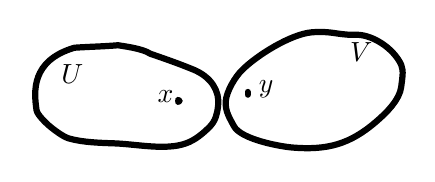
\begin{tikzpicture}[x=0.75pt,y=0.75pt,yscale=-0.8,xscale=0.8]


\draw  [line width=2.25]  (224.44,126.96) .. controls (219.83,123.68) and (206.96,122.25) .. (205.12,121.85) .. controls (194.97,122.69) and (188.44,122.69) .. (178.82,123.35) .. controls (152.52,131.1) and (154.39,149.97) .. (155.98,160.92) .. controls (156.39,163.75) and (161.97,169.05) .. (164.28,170.93) .. controls (165.91,172.26) and (171.78,176.91) .. (175.36,177.95) .. controls (183.78,180.38) and (194.17,180.63) .. (203.04,180.95) .. controls (216.42,181.44) and (233.91,185.31) .. (245.95,180.95) .. controls (251.7,178.87) and (255.95,175.14) .. (259.79,171.44) .. controls (263.87,167.5) and (264.7,163.37) .. (265.32,158.41) .. controls (266.44,149.5) and (261.25,140.86) .. (250.1,136.37) .. controls (244.45,134.1) and (239.14,131.99) .. (224.44,126.96) -- cycle ;

\draw  [line width=2.25] [line join = round][line cap = round] (241.29,154.82) .. controls (242.47,154.82) and (242.47,155.94) .. (241.29,155.94) ;

\draw  [line width=2.25] [line join = round][line cap = round] (283.12,149.98) .. controls (283.12,151.38) and (283.12,152.57) .. (283.12,151.18) ;

\draw  [line width=2.25]  (346.91,115.59) .. controls (337.26,115.59) and (333.41,113.15) .. (321.97,114.04) .. controls (309.18,115.03) and (288.4,128.06) .. (279.72,136.87) .. controls (275.62,140.79) and (270.45,149.55) .. (269.93,155.48) .. controls (269.4,161.54) and (272.49,166.06) .. (274.81,170.5) .. controls (279.05,178.61) and (302.95,182.87) .. (310.04,183.45) .. controls (331.33,185.19) and (344.79,181.39) .. (360.46,167.91) .. controls (366.25,162.94) and (374.78,154.86) .. (375.64,146.67) .. controls (376.06,142.68) and (377.29,137.4) .. (375.64,133.72) .. controls (371.01,123.41) and (357.25,114.6) .. (346.91,115.59) -- cycle ;

% Text Node
\draw (227,147.4) node [anchor=north west][inner sep=0.75pt]    {$x$};
% Text Node
\draw (288,141.4) node [anchor=north west][inner sep=0.75pt]    {$y$};
% Text Node
\draw (169,131.4) node [anchor=north west][inner sep=0.75pt]    {$U$};
% Text Node
\draw (343,118.4) node [anchor=north west][inner sep=0.75pt]    {$V$};


\end{tikzpicture}
\caption{Hausdorff space}
    \end{figure}
\end{propositionenv}
\begin{proofenv}
    \ \newline
    ``$\Rightarrow$'': If $(x,y)\in X\times X$, $x\neq y$, then $(x,y)\in (X\times X)\backslash \Delta_X$. There exists $ (U,V)\subseteq (X\times X)\backslash \Delta_X$, such that $(x,y)\in U\times V$, so $(U\times V)\cap \Delta_X=\varnothing$. Thus $U\cap V=\varnothing$. (If $p\in U\cap V$, then $(p,p)\in (U\times V)\cap \Delta_X$.)
    \newline
    ``$\Leftarrow$'': For any $(x,y)\in X\times X$, $x\neq y$, $\exists U\in \mathscr{T}$, $\forall V\in \mathscr{T}$, $x\in U, y\in V, U\cap V=\varnothing$. Then $(x,y)\in U\times V$ and $(U\times V)\cap \Delta_X=\varnothing$. So $\Delta_X$ is closed. 
\end{proofenv}
\begin{propositionenv}
    Let $(X,\mathscr{T})$ be a Hausdorff space. Let $\mathcal{F}$ be a non-degenerate filter on $X$. If $\mathcal{F}$ has a limit point\footnote{Let $(X,\mathscr{T})$ be a topological space and $\mathcal{F}$ be a filter on $X$. If $p\in X$ is such that $\mathcal{V}_p(\mathscr{T})\subseteq \mathcal{F}$, then we say that $p$ is a limit point of $\mathcal{F}$.}, then its limit point is unique.
\end{propositionenv}
\begin{proofenv}[By contradiction]
    Suppose that $x$ and $y$ are limit points of $\mathcal{F}$, $x\neq y$. Since $X$ is Hausdorff, $\exists (U,V)\in \mathscr{T}^2$, $x\in U,y\in V, U\cap V=\varnothing$. Since $x$ and $y$ are limit points of $\mathcal{F}$, $U\in\mathcal{F}, V\in \mathcal{F}$. This contradicts the hypothesis that $\mathcal{F}$ is non-degenerate.
\end{proofenv}
\begin{exampleenv}
    Any {\color{brown} metric space} is Hausdorff. 
    \newline
    Let $(X,\dd)$ be a metric space, $\forall (x,y)\in X\times X$, $x\neq y$, $\dd(x,y)>0$. Let $\varepsilon=\frac{\dd(x,y)}{2}$. $B(x,\varepsilon)\cap B(y,\varepsilon)=\varnothing.$ In fact, if $z\in B(x,\varepsilon)\cap B(y,\varepsilon)$,
    $$\dd(x,y)\le \dd(x,z)+\dd(z,y)<2\varepsilon=\dd(x,y).$$
\end{exampleenv}
\begin{propositionenv}
    Let $(X,\mathscr{T})$ be a topological space, $Y$ be a subset of $X$ and $p\in X$.
    \newline
    (1) Let $Z$ be a set and $f:Z\longrightarrow X$ be a mapping. Let $\mathcal{F}$ be a non-degenerate filter on $Z$. If $p$ is a limit of $f$ along $\mathcal{F}$, and if $f(Z)\subseteq Y$, then $p\in \overline{Y}$.
    \newline
    (2) Suppose that $p$ has a countable neighborhood basis. If $p\in \overline{Y}$, then there exists a sequence $(y_n)_{n\in\NN}$ in $Y$ that converges to $p$.
\end{propositionenv}
\begin{proofenv}
    \ \newline
    (1) $p$ is a limit of $f$ along $\mathcal{F}$ if and only if $\mathcal{V}_p(\mathscr{T})\subseteq f_*(\mathcal{F})$, or equivalently 
    $$\forall U\in \mathcal{V}_p(\mathscr{T}), f^{-1}(U)\in \mathcal{F}.$$
    $f(f^{-1}(U))\subseteq U\cap Y$, since $f(X)\subseteq Y$. Hence $U\cap Y\neq \varnothing$. So $p\in \overline{Y}.$
    \newline
    (2) Since $p$ has a countable neighborhood basis, there exists a decreasing sequence $V_0\supseteq V_1\supseteq\ldots$ of neighborhood of $p$ such that $\{V_n\mid n\in \NN\}$ forms a filter basis of $\mathcal{V}_p(\mathscr{T})$. For any $n\in \NN$, $V_n\cap Y=\varnothing$, we take $y_n\in V_n\cap Y$. The sequence $(y_n)_{n\in \NN}$ converges to $p$ since $\forall n\in \NN$, $\{y_k\mid k\in\NN,k\ge n\}\subseteq V_n$.
\end{proofenv}
\begin{exampleenv}
    Let $(X,\dd)$ be a semimetric space. $Y\subseteq X$, $\varepsilon>0$. If $(y_n)_{n\in\NN}$ is a sequence in $B(Y,\varepsilon)$, that converges to some $p\in X$, then 
    $$\lim_{n\rightarrow \infty}\dd(y_n,Y)=\dd(p,Y).$$
    Therefore, $\overline{B(Y,\varepsilon)}\subseteq \overline{B}(Y,\varepsilon):=\{x\in X\mid \dd(x,Y)\le \varepsilon\}$.
\end{exampleenv}
\begin{propositionenv}
    Let $(X,\dd)$ be a semimetric space, $Y\subseteq X$ be a closed subset. $\forall x\in X\backslash Y$, $\dd(x,Y)>0$.
\end{propositionenv}
\begin{proofenv}
    $X\backslash Y$ is open, so $\exists \varepsilon>0$ such that $B(X,\varepsilon)\subseteq{ X\backslash Y}$. So $\forall y\in Y$, $\dd(x,y)\ge \varepsilon$. Hence, $\dd(x,y)\ge \varepsilon$.
\end{proofenv}
\begin{corollaryenv}
    Let $(V,\pl\cdot\pl)$ be a semimetric space, $W$ be a closed vector subspace of $V$. $Q=V/W$. Then the quotient seminorm 
    $$\pl\cdot\pl_Q:Q\longrightarrow R,$$
    $$\alpha\longmapsto \inf_{x\in V,[x]=\alpha}\pl x\pl$$
    is a norm.
\end{corollaryenv}
\begin{proofenv}
    Let $\alpha\in Q\backslash{\alpha}$ and $x\in V$ such that $\alpha=[x]$. Since $\alpha\neq0, x\notin W$.
    $$0<\dd(x,W)\coloneq\inf_{y\in W}\pl x-y\pl=\inf_{\underset{[x']=\alpha}{x'\in V}}\pl x'\pl=\pl \alpha\pl_Q.$$
\end{proofenv}
\begin{propositionenv}
    If $(X,\mathscr{T})$ is a Hausdorff space, then, $\forall x\in X$, $\{x\}$ is closed.
\end{propositionenv}
\begin{proofenv}
    $\forall y\in X\backslash\{x\}$, $y\neq x$. So $\exists (U,V)\in \mathscr{T}\times\mathscr{T}$, $x\in U$, $y\in V$. $U\cap V=\varnothing$. So $V\subseteq X\backslash\{x\}$. Hence $X\backslash\{x\}$ is a neighborhood of $y$. 
\end{proofenv}
\begin{remark}
    Let $(V,\pl \cdot\pl)$ be a seminorm space. $W\subseteq V$, $Q=V/W$ and $\pl\cdot\pl_Q$ is the quotient seminorm. The mapping $\pi:V\longrightarrow Q, x\longmapsto [x]$  is continuous since $\pl[x]\pl_Q\le \pl x\pl$. If $\pl\cdot\pl_Q$ is a norm then $\{0_Q\}$ is closed (since $Q$ is Hausdorff). So $W=\pi^{-1}(\{0_Q\})=\ker(\pi)$ is closed. This shows that $\pl\cdot\pl_Q$ is a norm $\Leftrightarrow$ $W$ is closed.
\end{remark}



\section{Completeness}
\begin{definitionenv}
    Let $(X,\dd)$ be a semimetric space, $Y\subseteq X$, we define the diameter of $Y$ as $ \mathrm{diam}(Y)\coloneq\sup_{(x,y)\in Y^2}\dd(x,y)$. If $\mathrm{diam}(Y)<+\infty$, we say that $Y$ is \textbf{bounded}.
\end{definitionenv}
\begin{remark}
    Let $(E,\dd)$ be a semimetric space. 
    \newline
    (1) If $A$ and $B$ are subsets of $E$, then 
    $$A\subseteq B\Rightarrow \diam(A)\le \diam(B).$$
    (2) If $A\subseteq B\subseteq E$ and $B$ is bounded, then $A$ is bounded.
    \newline
    (3) If $A=\{x_1,\dots,x_n\}\subseteq E$, $n\in\NN_{\ge1}$. Then 
    $$\diam(A)=\max_{(i,j)\in \{1,\dots,n\}^2}\dd(x_i,x_j)<+\infty.$$
    So $A$ is bounded.
    \newline
    (4) $\forall p\in X$, $\diam(\bar{B}(p,r))\le 2r$, $\forall r\in \RR_{>0}$. In fact, $\forall (x,y)\in \bar{B}(p,r)^2$, $\dd(x,y)\le\dd(x,p)+\dd(p,y)\le 2r$.
\end{remark}
\begin{propositionenv}
    Let $(E,\dd)$ be a semimetric space, $A\subseteq E$. Suppose that $A$ is bounded. Let $r=\diam(A)$. For any $p\in A$, $A\subseteq\bar{B}(p,r)$.
\end{propositionenv}
\begin{proofenv}
    $\forall x\in A,\ \dd(p,x)\le \diam(A)=r.$
\end{proofenv}
\begin{propositionenv}\label{8.7.4}
    Let $(E,\dd)$ be a semimetric space, $A\subseteq E$, $B\subseteq E$ and $(x_0,y_0)\in A\times B$. Then 
    $$\diam(A\cup B)\le \diam(A)+\diam(B)+\dd(x_0,y_0).$$
\end{propositionenv}
\begin{proofenv}
    Let $(x,y)\in \left(A\cup B\right)^2$.
    \newline
    Case 1. $\{x,y\}\in A$, $\dd(x,y)\le \diam(A)$.
    \newline
    Case 2. $\{x,y\}\in B$, $\dd(x,y)\le \diam(B)$.
    \newline
    Case 3. $x\in A,\ y\in B,$
    $$\dd(x,y)\le \dd(x,x_0)+\dd(x_0,y_0)+\dd(y_0,y)\le \diam(A)+\diam(B)+\dd(x_0,y_0).$$
    Case 4. $x\in B,\ y\in A$. Same as case 3.
    \begin{figure}[H]
        \centering


\tikzset{every picture/.style={line width=0.75pt}} %set default line width to 0.75pt        

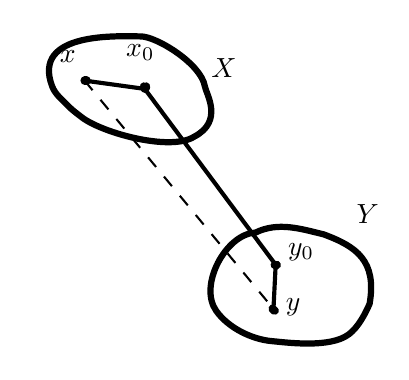
\begin{tikzpicture}[x=0.75pt,y=0.75pt,yscale=-1,xscale=1]
%uncomment if require: \path (0,300); %set diagram left start at 0, and has height of 300

%Shape: Regular Polygon [id:dp2830885640667714] 
\draw  [line width=2.25]  (178.45,40.02) .. controls (168.57,40.02) and (125.53,37.32) .. (135.86,64.18) .. controls (137.33,68.01) and (140.8,70.66) .. (143.6,73.58) .. controls (145.55,75.6) and (147.85,77.23) .. (150.05,78.95) .. controls (159.66,86.44) and (192.79,95.62) .. (204.26,88.34) .. controls (218.6,80.85) and (209.98,67.67) .. (209.42,64.18) .. controls (207.67,53.24) and (186.09,40.02) .. (178.45,40.02) -- cycle ;
%Shape: Regular Polygon [id:dp5369449128522238] 
\draw  [line width=2.25]  (233.77,134.54) .. controls (219.59,135.17) and (206.11,160.06) .. (214.89,172.29) .. controls (220.91,180.68) and (232.32,186.08) .. (241.98,186.87) .. controls (247.51,187.32) and (269.81,190.58) .. (278.92,183.44) .. controls (283.42,179.91) and (286.55,173.88) .. (288.77,168.85) .. controls (292.34,148.12) and (282.49,141.26) .. (266.61,135.4) .. controls (255.4,132.68) and (244.73,129.25) .. (233.77,134.54) -- cycle ;
%Shape: Free Drawing [id:dp9278093506246873] 
\draw  [line width=3] [line join = round][line cap = round] (181.06,64.14) .. controls (181.06,65.64) and (180.06,65.64) .. (180.06,64.14) ;
%Shape: Free Drawing [id:dp5177768898138636] 
\draw  [line width=3] [line join = round][line cap = round] (243.06,150.14) .. controls (243.4,150.14) and (244.06,150.47) .. (244.06,150.14) ;
%Shape: Free Drawing [id:dp9393552590803542] 
\draw  [line width=3] [line join = round][line cap = round] (243.06,172.14) .. controls (242.59,172.14) and (242.06,171.61) .. (242.06,171.14) ;
%Straight Lines [id:da5018713202956172] 
\draw [line width=1.5]    (151.45,61.32) -- (180.45,65.32) ;
%Shape: Free Drawing [id:dp8007345261566203] 
\draw  [line width=3] [line join = round][line cap = round] (151.45,61.32) .. controls (151.78,61.32) and (152.12,61.32) .. (152.45,61.32) ;
%Straight Lines [id:da12265525507083463] 
\draw [line width=1.5]    (180.45,65.32) -- (244.45,151.32) ;
%Straight Lines [id:da35248354429149964] 
\draw [line width=1.5]    (243.45,151.32) -- (242.45,171.32) ;
%Straight Lines [id:da8163970346630994] 
\draw  [dash pattern={on 4.5pt off 4.5pt}]  (151.45,61.32) -- (242.45,171.32) ;

% Text Node
\draw (211,49.4) node [anchor=north west][inner sep=0.75pt]    {$X$};
% Text Node
\draw (281,119.4) node [anchor=north west][inner sep=0.75pt]    {$Y$};
% Text Node
\draw (138,45.4) node [anchor=north west][inner sep=0.75pt]    {$x$};
% Text Node
\draw (170,42.4) node [anchor=north west][inner sep=0.75pt]    {$x_{0}$};
% Text Node
\draw (248,138.4) node [anchor=north west][inner sep=0.75pt]    {$y_0$};
% Text Node
\draw (246.95,164.72) node [anchor=north west][inner sep=0.75pt]    {$y$};


\end{tikzpicture}
\caption{proposition. \ref{8.7.4}}
    \end{figure}
\end{proofenv}
\begin{corollaryenv}
    If $A\cap B\neq\varnothing$, then 
    $$\diam(A\cup B)\le \diam(A)+\diam(B).$$
\end{corollaryenv}
\begin{definitionenv}
    Let $(E,\dd)$ be a semimetric space, and $\mathcal{F}$ be a non-degenerate filter on $E$. If $\inf_{A\in \mathcal{F}}\diam(A)=0$, we say that $\mathcal{F}$ is a \textbf{Cauchy filter}.
\end{definitionenv}
\begin{exampleenv}
    $E=\interval[open left]{0}{1}$. If $\mathcal{F}$ is generated by $\interval[open]{0}{\varepsilon}$, $\varepsilon\le 1$, then $\mathcal{F}$ is a Cauchy filter.
\end{exampleenv}
\begin{propositionenv}
    Let $(E,\dd)$ be a semimetric space and $\mathcal{F}$ be a non-degenerate filter on $E$. If $\mathcal{F}$ has a limit point $p$, then $\mathcal{F}$ is a Cauchy filter.
\end{propositionenv}
\begin{proofenv}
    $\forall \varepsilon>0$, $\bar{B}(p,\frac{\varepsilon}{2})\in \mathcal{F}$, $\diam(\bar{B}(p,\frac{\varepsilon}{2}))\le \varepsilon$. So $\dis \inf_{A\in \mathcal{F}}\diam(A)=0.$
\end{proofenv}
\begin{propositionenv}
    Let $(E,\dd)$ be a semimetric space, and $\mathcal{F}$ be a Cauchy filter on $E$. Any adherent point of $\mathcal{F}$ is a limit point of $\mathcal{F}$.
\end{propositionenv}
\begin{proofenv}
    Let $\varepsilon>0$. Let $A\in \mathcal{F}$ such that $\diam(A)<\frac{\varepsilon}{2}$. Note that $B(p,\frac{\varepsilon}{4})\cap A\neq\varnothing$. So 
    $$\diam(B(p,\frac{\varepsilon}{4})\cup A)\le \diam(B(p,\frac{\varepsilon}{4}))+\diam(A)<\frac{\varepsilon}{2}+\frac{\varepsilon}{2}.$$
    So $A\subseteq B(p,\varepsilon)$.
\end{proofenv}
\begin{definitionenv}
    Let $(E,\dd)$ be a semimetric space. $I\subseteq \NN$ be an infinite subset, $\mathcal{F}$ be the Fréchet filter on $I$. We say that a sequence $x\coloneq (x_n)_{n\in I}\in E^I$ is a Cauchy sequence if $x_*(\mathcal{F})\coloneqq\{U\subseteq E\mid x^{-1}(U)\in \mathcal{F}\}$ is a Cauchy filter. Or equivalently,
    $$\forall \varepsilon>0,\ \exists N\in I,\ \forall n,m\in I^2_{\ge N},\ \dd(x_n,x_m)\le \varepsilon.$$
\end{definitionenv}
\begin{proofenv}
    ``$\Rightarrow$'' $\forall \varepsilon>0,\ \exists U\in x_*(\mathcal{F}),\ \diam(U)\le\varepsilon$. Since $x^{-1}(U)\in \mathcal{F}$, $\exists N\in \NN$ such that $I_{\ge N}\subseteq x^{-1}(U)$. So $\{x_n\mid n\in I_{\ge N}\}\subseteq U$, which leads to 
    $$\forall (n,m)\in I_{\ge N}^2,\ \dd(x_n,x_m)\le \varepsilon.$$
    ``$\Leftarrow$'' $\forall \varepsilon>0,\ \exists N\in \NN$, $\diam\left(\{x_n\mid n\in I_{\ge N}\}\right)\le \varepsilon$.
\end{proofenv}
\begin{propositionenv}
    Let $(E,\dd)$ be a semimetric space, and $(x_n)_{n\in I}$ be a sequence in $E$.
    \newline
    (1) If $(x_n)_{n\in I}$ is convergent, then it is a Cauchy sequence.
    \newline
    (2) If $(x_n)_{n\in I}$ is a Cauchy sequence, then $\{x_n\mid n\in I\}$ is bounded.
    \newline
    (3) If $(x_n)_{n\in I}$ is a Cauchy sequence, then any of its subsequence is a Cauchy sequence.
    \newline
    (4) If $(x_n)_{n\in I}$ is a Cauchy sequence, and if there exists a subsequence $(x_n)_{n\in J}$ that converges to some $p\in E$, then $(x_n)_{n\in I}$ converges to $p$.
\end{propositionenv}
\begin{proofenv}
    Let $\mathcal{F}_I$ be a Fréchet filter on $I$.
    \newline
    (1) $x_*(\mathcal{F}_I)$ has a limit point. So it is a Cauchy filter. 
    \newline
    (2) $\exists N\in \NN$ such that $\diam(\{x_n\mid n\in I_{\ge \NN}\})\le 1<+\infty$. So $\diam\left(\{x_n\mid n\in I\}\right)<+\infty$ since
    $$\{x_n\mid n\in I\}=\{x_n\mid n\in I_{< N}\}\cup\{x_n\mid n\in I_{\ge N}\}.$$
    (3) Let $J$ be an infinite subset of $I$, $\lambda:J\longrightarrow I$ be the inclusion mapping, and $\mathcal{F}_J$ be the Fréchet filter. Then $\lambda_*(\mathcal{F}_J)\supseteq \mathcal{F}_I$.
    $$(x\circ \lambda)_*(\mathcal{F}_J)=x_*(\lambda_*(\mathcal{F}_J))\supseteq x_*(\mathcal{F}_I.)$$
    Since $x_*(\mathcal{F}_I)$ is a Cauchy filter, $(x\circ \lambda)_*(\mathcal{F}_J)$ is a Cauchy filter.
    \newline
    (4) We keep the notation introduced in the proof of (3). If $p$ is a limit point of $x\circ \lambda_*\left(\mathcal{F}_J\right)$. Then $p$ is an adherent point of $x_*(\mathcal{F}_I)$. Since $x_*(\mathcal{F}_I)$  is a Cauchy filter, $p$ is a limit point of $x_*(\mathcal{F}_I)$. 
\end{proofenv}
\begin{definitionenv}
    Let $(X,\dd)$ be a semimetric space. If any Cauchy filter on $X$ has a limit point, then we say that $(X,\dd)$ is complete.
\end{definitionenv}
\begin{propositionenv}
    Let $(X,\dd)$ be a {\color{brown} metric space} and $Y$ be a subset of $X$. If $(Y,\dd)$ is complete, then $Y$ is a closed subset of $X$.
\end{propositionenv}
\begin{proofenv}
    Let $(y_n)_{n\in\NN}$ be a sequence in $Y$ that converges in $X$ to some $p\in X$. So $(y_n)_{n\in \NN}$ is a Cauchy sequence in $Y$, thus it converges to some $q\in Y$. Since $X$ is Hausdorff, $p=q$. Then $\bar{Y}=Y$ (Since $\bar{Y}$ is the set of limits of all sequence in $Y$). So $Y$ is closed.
\end{proofenv}
\begin{exampleenv}
    $(\RR,\left|\ \cdot\ \right|)$ is complete.
    \newline
    Let $(x_n)_{n\in I}$ be a Cauchy sequence in $\RR$. Let $M>0$ such that $\forall n\in I, |x_n|\le M$. Hence,
    $$ -M\le \liminf_{n\rightarrow +\infty} x_n\le \limsup_{n\rightarrow +\infty}x_n\le M.$$
    By Bolzano-Weierstrass, $\exists J\subseteq I$ infinite such that $(x_n)_{n\in I}$ converges to $\limsup_{n\rightarrow +\infty}x_n\in \RR$. So $(x_n)_{n\in I}$ converges.
\end{exampleenv}
\begin{propositionenv}
    Let $(X,\dd)$ be a semimetric space, $(X,\dd)$ is complete if and only if any Cauchy sequence in $X$ is convergent.
\end{propositionenv}
\begin{proofenv}
    It is suffices to prove ``$\Leftarrow$''. Suppose that all Cauchy sequence in $X$ converges. Let $\mathcal{F}$ be a Cauchy filter on $X$. 
    $\forall n\in \NN$, let $A_n\in \mathcal{F}$, $\diam(A)<\frac{1}{n+1}$. $\forall n\in \NN$, let $B_n=A_0\cap\ldots\cap A_n\in \mathcal{F}$, $\diam(B)\le \frac{1}{n+1}$. Take $x_n\in B_n$. Then $(x_n)_{n\in \NN}$ is a Cauchy sequence. Hence $(x_n)_{n\in \NN}$ converges to $p\in X$. 
    
    \quad We claim that $p$ is a limit point of $\mathcal{F}$. If $V$ is a neighborhood of $p$, then $\exists N\in \NN$ such that $\{x_n\mid  n\in \NN_{\ge N}\}\subseteq V$. So $V\cap B_n\neq\varnothing, \ \forall n \in \NN_{\ge N}$.
    
    \quad Let $A\in \mathcal{F}$, $A\cap B_n\neq\varnothing$. Take $y_n\in A\cap B_n$, $(y_n)_{n\in\NN}$ is a Cauchy sequence. $\dd(y_n,x_n)\le\frac{1}{1+n}$, so $(y_n)_{n\in \NN}$ converges to $p$. Thus $V\cap A\neq \varnothing$.
\end{proofenv}
\begin{propositionenv}
    Let $n$ be a positive integer. For any $i\in\{1,\ldots,n\}$, let $(X_i,\dd_i)$ be a semimetric space. Let $X=X_1\times\ldots\times X_n$ and 
    $$\pi_i:X\longrightarrow X_i$$
    $$(x_1,\ldots,x_n)\longmapsto x_i$$
    be the projection mapping. We equip $X$ with the product semimetric $\dd$
    $$\dd((x_1,\ldots,x_n),(y_1,\ldots,y_n))\coloneqq \max_{i\in\{1,\ldots,n\}}\dd_i(x_i,y_i).$$
    Let $\mathcal{F}$ be a non-degenerate filter on $X$. For any $i\in\{1,\ldots, n\}$, let
    $$\mathcal{F}_i=\left(\pi_i\right)_{*}\left(\mathcal{F}\right).$$ 
    (1) The filter $\mathcal{F}$ is a Cauchy filter if and only if $\mathcal{F}_i$ is a Cauchy filter for any $i\in \{1,\ldots,n\}$.
    \newline
    (2) The filter $\mathcal{F}$ has a limit point if and only if $\mathcal{F}_i$ has a limit point for any $i\in \{1,\ldots,n\}$. If $p_i$ is the limit point of $\mathcal{F}_i$, then $p=\left(p_1,\ldots,p_n\right)$ is a limit point of $\mathcal{F}$.
    \newline
    (3) If $\left(X_1,\dd_1\right),\ldots,\left(X_n,\dd_n\right)$ are complete, then $(X,\dd)$ is complete.
\end{propositionenv}
\begin{proofenv}
    \ \newline
    (1)
    Since $\pi_i$ are Lipschitzian, if $\mathcal{F}$ is a Cauchy filter, then $\mathcal{F}_i$  are all Cauchy filters. Conversely, let $\mathcal{F}$ be a non-degenerate filter such that $\mathcal{F}_i$ is a Cauchy filter for all $i\in\{1,\ldotp,n\}$. For any $\varepsilon>0$, any $i\in\{1,\ldots,n\}$, there exists $A_i\in \mathcal{F}_i$ such that $\diam(A_i)<\varepsilon$. We define 
    $$A\coloneqq A_1\times\ldots\times A_n=\bigcap_{i=1}^n\pi_{i}^{-1}\left(A_i\right)\in\mathcal{F}.$$
    For any $\left(x_1,\ldots,x_n\right),\left(y_1,\ldots,y_n\right)\in A$, $\dis\dd(x,y)=\max_{i\in\{1,\ldots,n\}}\dd_{i}(x_i,y_i)<\varepsilon.$
    \newline
    (2) $\pi_i$ is Lipschitzian so also continuous $i\in \{1,\ldots,n\}$, therefore, if $p=(p_1,\ldots,p_n)$ a limit point of $\mathcal{F}$, then $\pi_i(p)=p_i$ is a limit point of $\mathcal{F}_i$. 
    
    \quad Conversely, Suppose that $p_i$ is a limit point of $\mathcal{F}_i$. Let $U$ be a neighborhood of $p$. There exists $U_i\in\mathcal{F}_i$ neighborhood of $p_i$ such that $U_1\times \ldots\times U_n\subseteq U$.
    $$U\supseteq \bigcap_{i=1}^n\pi_{i}^{-1}\left(U_i\right)\in\mathcal{F},$$
    so $U\in\mathcal{F}$.
\end{proofenv}
\begin{propositionenv}
    Let $(X,\dd_X)$, $(Y,\dd_Y)$ be two semimetric spaces, $f:X\longrightarrow Y$ be uniformly continuous. For any Cauchy filter $\mathcal{F}$ on $X$, $f_*(\mathcal{F})$ is also a Cauchy filter on $Y$.
\end{propositionenv}
\begin{proofenv}
    $\forall \varepsilon>0,\ \exists \delta>0$ such that 
    $$\forall (x,y)\in X\times X,\ \dd_X(x,y)<\delta\Rightarrow \dd_Y(f(x),f(y))<\varepsilon.$$
    Let $A\in \mathcal{F}$ such that $\diam(A)<\delta$, then $f(A)\in f_*(\mathcal{F})$ and $\diam(f(A))<\varepsilon$.
\end{proofenv}
\begin{propositionenv}
    Let $(X,\dd),(X',\dd')$ be two semimetric spaces, $f:X\longrightarrow X'$ injective mapping. Assume that there exists positive constants $C_1$ and $C_2$ such that $\forall (x,y)\in X\times X$, $C_1\cdot \dd(x,y)\le \dd'\left(f(x),f(y)\right)\le C_2\cdot\dd(x,y)$. 
    \newline
    (1) For any sequence $(x_i)_{i\in I}$ in $X$, the sequence $(x_i)_{i\in I}$ is a Cauchy sequence if and only if the sequence $\left(f(x_i)\right)_{i\in I}$ is a Cauchy sequence.
    \newline
    (2) For any $(x_i)_{i\in I}$ in $X$, $(x_i)_{i\in I}$ is a convergent if and only if $\left(f(x_i)\right)_{i\in I}$ is convergent.
    \newline
    (3) If $(X,\dd)$ is complete, then $(f(X),\dd')$ is complete. $f(X)$ is closed in $X'$ if in addition we assume that $\dd'$ is a metric.
\end{propositionenv}
\begin{proofenv}
    Note that $f:X\longrightarrow f(X)$, $f^{-1}: f(X)\longrightarrow X$ are Lipschitzian. Apply the previous proposition.
\end{proofenv}
\begin{theoremenv}
    Let $(K,\left|\ \cdot\ \right|)$ be a valued filed such that $\left(K,\left|\ \cdot\ \right|\right)$ is complete. Let $V$ be a finite dimensional vector space over $K$. 
    \newline
    (1) All possible norms on $K$ are equivalent.
    \newline
    (2) For any norm $\pl\cdot\pl $ on $V$, the normed space $\left(V,\pl\cdot\pl\right)$ is complete.
    \newline
    (3) If we equip $V$ with the topology induced by an arbitrary norm $\pl\cdot\pl$. For any normed vector space $\left(V,\pl\cdot\pl\right)$, any $K$-linear mapping $f:V\longrightarrow V'$ is bounded and $f\left(V\right)$ is closed in $V'$.
\end{theoremenv}
\begin{proofenv}
    Let $e\coloneq \left(e_i\right)_{i=1}^n$ be a basis of $V$. Then, the mapping
    $$\pl\cdot\pl_e: V\longrightarrow \RR_{>0},\ \pl a_1e_1+\ldots+ a_ne_n\pl=\max_{i\in\{1,\ldots,n\}}\left|e_i\right|$$
    is a norm on $V$. For $f:V\longrightarrow V'$, 
    \begin{align}
        \pl f\left(a_1e_1+\ldots+a_ne_n\right)\pl'&=\pl a_1 f\left(e_1\right)+\ldots+ a_nf\left(e_n\right)\pl'\\
        &\le\left|a_1\right|\pl f\left(e_1\right)\pl' +\ldots+\left|a_n\right|\pl f\left(e_n\right)\pl'\\
        &\le \max_{i\in\{1,\ldots,n\}}\left|a_i\right|\sum_{i=1}^{n}\pl f\left(e_i\right)\pl'.
    \end{align}
    Therefore the $K$-linear mapping $f:\left(V,\pl\cdot\pl_e\right)\longrightarrow \left(V',\pl\cdot\pl'\right)$ is bounded. In particular, for any $\pl\cdot\pl$ on $V$, 
    $\mathrm{Id}: \left(V,\pl\cdot\pl\right)\longrightarrow \left(V,\pl\cdot\pl\right)$ is bounded. So there exists $C>0$, $\pl\cdot\pl\le C\pl\cdot\pl_e$.

    \quad To prove the theorem, we reason by induction with respect to $n=\dim\left(V\right)$. 
    
    \quad In case when $n=0$, $V=\{0\}$ has the unique norm $\pl\cdot\pl_0$ (constant mapping with the value $0\in \RR$). Any sequence in $\{0_V\}$ is constant, and hence convergent ($\left(\{0\},\pl\cdot\pl_0\right)$ complete). If $f:\left(\{0_V\},\pl\cdot\pl\right)\longrightarrow \left(V,\pl\cdot\pl\right)$ is $K$-linear, then it is bounded. The unique $f\left(\{0_V\}\right)$ is a one-point set, which is closed, since $\left(V,\pl\cdot\pl\right)$ is Hausdorff. 

    \quad In case when $n=1$, let $e_1$ be the basis of $V$, and $\pl\cdot\pl$ be an arbitrary norm on $V$.
    $$\pl a_1e_1\pl =\left|a_1\right|\pl e_1\pl=\pl a_1e_1\pl_{e_1}\cdot\pl e_1\pl, $$
    so $\pl\cdot\pl$ is equivalent to $\pl\cdot\pl_{e_1}$.
    \newline
    (2) Since $(K,\left|\ \cdot\ \right|)$ is complete, so $(V,\pl\cdot\pl_{e_1})$ is also complete, since 
    $$(K,\left|\ \cdot\ \right|)\longrightarrow (V,\pl\cdot\pl_{e_1})$$
    $$a\longmapsto ae_1$$
    is an isomorphism.
    \newline
    (3) We have seen that the mapping $f:\left(V,\pl\cdot\pl_{e_1}\right)\longrightarrow \left(V',\pl\cdot\pl'\right)$ is bounded. So $f:\left(V,\pl\cdot\pl\right)\longrightarrow \left(V',\pl\cdot\pl'\right)$ is also bounded. $f(V)=\{0\}$, or $(f(V),\pl\cdot\pl')$ is of dimension $1$, so $(f(V),\pl\cdot\pl')$ is complete, so $f(V)$ is closed.
    \newline
    Suppose that the theorem holds for normed vector space of dimension $<n$. Then the case of dimension $n$:

    \quad Let $e=(e_i)_{i=1}^n$ be a basis of $V$. Let $W=\mathrm{span}_K\left(\{e_1,\ldots,e_n\}\right)$. If $\pl\cdot\pl$ is a norm on $V$, then, by the induction hypothesis,
    
    (i) $\pl\cdot\pl$ and $\pl\cdot\pl_{\underline{e}}$ are equivalent on $W$, that is, $\exists A>0$ such that $\forall(a_1,\ldots,a_{n-1})$, 
    $$\max\{|a_1|,\ldots,|a_n|\}=\pl a_1e_1+\ldots+a_{n-1}e_{n-1}\pl_{\underline{e}}\le A\pl a_1e_1+\ldots+a_{n-1}e_{n-1}\pl.$$ 
    (ii) $(W,\pl\cdot\pl)$ is complete.

    (iii) $W$ is a closed subset of $V$.

    Let $Q=V/W$, and $\pl\cdot\pl_Q$ be the quotient norm on $Q$. Let $(b_1,\ldots,b_n)\in K^n,$
    $$s=b_1e_1+\ldots+b_ne_n\in V,\ t=b_1e_1+\ldots+b_ne_n+w\in V,\ \alpha=[s]=b_n[e_n]\in Q.$$
    $$\pl t\pl =\pl s-b_ne_n\pl\le \pl s\pl+\left|b_n\right|\pl e_n\pl.$$
    Take $B=\frac{\pl e_n\pl}{\pl[e_n]\pl_Q}\in \RR$, $\pl s\pl\ge\pl\alpha\pl_Q=\left|b_n\right|\pl[e_n]\pl_Q=B^{-1}|b_n|\pl e_n\pl$.
    $$B^{-1}\pl s\pl\ge\left(\pl t\pl-|b_n|\cdot\pl e_n\pl\right)B^{-1}$$
    $$\pl s\pl \ge B^{-1}\cdot|b_n|\cdot\pl e_n\pl.$$
    $$\left(B^{-1}+1\right)\pl s\pl \ge B^{-1}\pl t\pl\ge B^{-1}A^{-1}\max\{|b_1|,\ldots,|b_n|\}$$
    Take $C=\min\left\{\frac{B^{-1}A^{-1}}{B^{-1}+1},B^{-1}\cdot\pl e_n\pl\right\}$. Then $\pl s\pl\ge C\max\{|b_1|,\ldots,|b_n|\}$. So $\pl\cdot\pl$ is equivalent to $\pl\cdot\pl_{\underline{e}}$.
    \newline
    (2) Since $(V,\pl\cdot\pl)_e$ is complete and $\pl\cdot\pl$ is equivalent to $\pl\cdot\pl_e$, we obtain that $(V,\pl\cdot\pl)$ is also complete.
    \newline
    (3) Since $f:\left(V,\pl\cdot\pl_e\right)\longrightarrow \left(V',\pl\cdot\pl'\right)$ is bounded, $f:\left(V,\pl\cdot\pl\right)\longrightarrow \left(V',\pl\cdot\pl'\right)$ is also bounded. 
    
    \quad If $f$ is not injective, $\dim\left(f(V)\right)<n$, so $\left(f(V),\pl\cdot\pl'\right)$ is complete, $f(V)$ is thus closed.

    \quad If $f$ is injective, then $\pl f(\cdot)\pl'$ and $\pl\cdot\pl$ are equivalent norms on $V$. So $\left(f(V),\pl\cdot\pl'\right)$ is complete. Hence $f(V)$ is closed.
    
\end{proofenv}
\begin{propositionenv}
    Let $(X,\dd)$ be a complete semimetric space. Let $Y\subseteq X$ be a closed subset. Then $(Y,\dd)$ is complete.
\end{propositionenv}
\begin{proofenv}
    Let $(x_n)_{n\in\NN}$ be a Cauchy sequence in $Y$. It is also a Cauchy sequence in $X$, so converges to some $l\in X$. Since $Y$ is closed, one has $l\in Y$. So $(Y,\dd)$ is complete.
\end{proofenv}


\section{Compactness}
\begin{definitionenv}
    Let $X$ be a set and $\mathcal{F}$ be a non-degenerate filter on $X$. If there does not exists any non-degenerate filter $\mathcal{G}$ on $X$ such that $\mathcal{F}\subsetneq\mathcal{G}$, then we say that $\mathcal{F}$ is an ultrafilter.
\end{definitionenv}
\begin{propositionenv}
    For any non-degenerate filter $\mathcal{F}$ on $X$, there exists an ultrafilter on $X$ containing $\mathcal{F}$.
\end{propositionenv}
\begin{proofenv}
    Let $\Theta$ be a set of non-degenerate filters containing $\mathcal{F}$, equipped with $\subseteq$. Let $\Theta_0$ be a non-empty totally ordered subset. Let $\dis \mathcal{F}'=\bigcup_{\mathcal{H}\in\Theta_0}\mathcal{H}$.
    
    We prove that $\mathcal{F}'$ is a filter.

    (1) Let $(V_1,V_2)\in \mathcal{F}'\times\mathcal{F}'$, $\exists \mathcal{H}_1,\mathcal{H}_2$ in $\Theta_0$, $V_1\in\mathcal{H}_1,\ V_2\in \mathcal{H}_2$. Since $\Theta_0$ is totally ordered, either $\mathcal{H}_1\subseteq\mathcal{H}_2$ or $\mathcal{H}_2\subseteq\mathcal{H}_1$. 

    If $\mathcal{H}_1\subseteq \mathcal{H}_2, V_1\cap V_2\in \mathcal{H}_2\subseteq\mathcal{F}'$. If $\mathcal{H}_2\subseteq\mathcal{H}_1,V_1\cap V_2\in \mathcal{H}_1\subseteq\mathcal{F}'$.

    (2) Let $V\in \mathcal{F}'$, let $\mathcal{H}\in \Theta_0$ such that $V\in \mathcal{H}$. $\forall U\in \wp(X), U\supseteq V$, one has $U\in \mathcal{H}\subseteq\mathcal{F}'$. So $\mathcal{F}'\in \Theta$. It is an upper bound of $\Theta_0$. By Zorn's lemma, there exists maximal $\mathcal{G}\in \Theta$, it is an ultrafilter containing $\mathcal{F}$.

\end{proofenv}
\begin{propositionenv}
    Let $X$ be a set and $\mathcal{F}$ be a non-degenerate filter on $X$. The following conditions are equivalent.
    \newline
    (1) $\mathcal{F}$ is an ultrafilter.
    \newline
    (2) $\forall A\in \wp(X)$, either $A\in \mathcal{F}$ or $X\backslash A\in \mathcal{F}$.
    \newline
    (3) $\forall (A,B)\in \wp(X)^2$, if $A\cup B\in \mathcal{F}$, then $A\in \mathcal{F}$ or $B\in\mathcal{F}$.
\end{propositionenv}
\begin{proofenv}
    \ \newline
    (1)$\Rightarrow $(2): Suppose that $A\in \wp(X)$ such that $A\notin \mathcal{F}$ and $X\backslash A\notin\mathcal{F}$. Let $B\in \mathcal{F}$. If $B\cap A=\varnothing$, then $B\subseteq X\backslash A$, $(X\backslash A)\in \mathcal{F}$. So $\mathcal{F}\cup\{A\}$ generates a non-degenerate filter $\mathcal{F}'\supsetneq\mathcal{F}$, contradiction.
    \newline
    (2)$\Rightarrow$(3): Suppose that $B\notin \mathcal{F}$. Then $X\backslash B\in \mathcal{F}$. So $\left(A\cup B\right)\cap \left(X\backslash B\right)\in \mathcal{F}$. So $A\in \mathcal{F}$.
    \newline
    (3)$\Rightarrow$(1): Let $\mathcal{F}'$ be a non-degenerate filter such that $\mathcal{F}\subsetneq\mathcal{F}'$. Take $A\in \mathcal{F}'\backslash \mathcal{F}$.

    Then $X=A\cup\left(X\backslash A\right)$. Since $A\notin\mathcal{F}$, $X\backslash A\in \mathcal{F}\subseteq \mathcal{F}'$. So $\varnothing=A\cap\left(X\backslash A\right)\in \mathcal{F}'$. Contradiction.
\end{proofenv}
\begin{corollaryenv}
    Let $f:X\longrightarrow Y$ be mapping of sets. If $\mathcal{F}$ is an ultrafilter on $X$, then $f_*(\mathcal{F})$ is an ultrafilter on $Y$.
\end{corollaryenv}
\begin{proofenv}
    Let $A$ and $B$ be subsets of $Y$ such that 
    $$A\cup B\in f_*(\mathcal{F}):=\{C\subseteq Y\mid f^{-1}(C)\in \mathcal{F}\}$$
    $$f^{-1}\left(A\cup B\right)=f^{-1}(A)\cup f^{-1}(B)\in \mathcal{F}.$$
    Since $\mathcal{F}$ is an ultrafilter, $f^{-1}(A)\in \mathcal{F}$ or $f^{-1}(B)\in \mathcal{F}$. Namely, $A\in f_*(\mathcal{F})$ or $B\in f_*(\mathcal{F})$.
\end{proofenv}
\begin{definitionenv}
    Let $(X,\mathscr{T})$ be a topological space, $Y\subseteq X$ and $\left(U_i\right)_{i\in I}$  be a family of subset of $X$.
    \newline
    (1) If $Y\subseteq\bigcup_{i\in I}U_i$, we say that $\left(U_i\right)_{i\in I}$ is a \textbf{cover} of $Y$.
    \newline
    (2) If $\exists J\in I$ such that $Y\subseteq \bigcup_{j\in J}U_j$, we say that $\left(U_j\right)_{j\in J}$ is a \textbf{subcover} of $\left(U_i\right)_{i\in I}$ of $Y$.
    \newline
    (3) If $\left(U_i\right)_{i\in I}\in \mathscr{T}^I$ is a cover of $Y$, we say that ti is an \textbf{open cover} of $Y$.
    \newline
    (4) If $I$ is a finite set and $\left(U_i\right)_{i\in I}$ is a cover of $Y$, we say that $\left(U_i\right)_{i\in I}$ is a \textbf{finite open cover}.
\end{definitionenv}
\begin{propositionenv}
    Let $\left(X,\mathscr{T}\right)$ be a topological space and $Y\subseteq X$. The following conditions are equivalent:
    \newline
    (1) For any ultrafilter $\mathcal{G}$ on $X$ such that $Y\in \mathcal{G}$, $\mathcal{G}$ has a limit point in $Y$.
    \newline
    (2) For any non-degenerate filter $\mathcal{F}$ on $X$, such that $Y\in \mathcal{F}$, $\mathcal{F}$ has an adherent point in $Y$.
    \newline
    (3) Any open cover of $Y$ has a finite subcover.
\end{propositionenv}
\begin{proofenv}
    \ \newline
    (1)$\Rightarrow$(2) Let $\mathcal{G}$ be an ultrafilter containing $\mathcal{F}$ and $x\in Y$ be a limit point of $\mathcal{G}$. For any $U\in \mathcal{V}_x\left(\mathscr{T}\right)$, $U\in \mathcal{G}$, so $\forall A\in \mathcal{F}$, $U\cap A\neq\varnothing$.
    \newline
    (2)$\Rightarrow$(1) Let $\mathcal{G}$ be an ultrafilter, and let $x\in Y$ be an adherent point of $\mathcal{G}$. Then the filter $\mathcal{G}'$ generated by $\mathcal{G}\cup\mathcal{V}_x(\mathscr{T})$ is non-degenerate and contains $\mathcal{G}$. So $\mathcal{G}'=\mathcal{G}$. This means $\mathcal{V}_x(\mathscr{T})\subseteq\mathcal{G}$.
    \newline
    (2)$\Rightarrow$(3) Let $(U_i)_{ i\in I}$ be an open cover of $Y$. Suppose that it does not have any finite subcover. For any $i\in I$, let $F_i=X\backslash U_i$. For any finite subset $J$ of $I$, $\dis Y\nsubseteq  \bigcup_{j\in J}U_j$. So
    $$Y\bigcap\left(X\backslash \bigcup_{j\in J}U_j\right)=Y\bigcap\left(\bigcap_{j\in J}F_j\right)\neq\varnothing.$$
    So $\{F_i\mid i\in I\}\cup\{Y\}$ generates a non-degenerate filter $\mathcal{F}$. It has an adherent point of $x\in Y$. Since $Y\subseteq \bigcup_{i\in I}U_i$, $\exists i_0\in I$, $x\in U_{i_0}$. So $U_{i_0}\in \mathcal{V}_x(\mathscr{T})$. This is impossible since $U_{i_0}\cap F_{i_0}=\varnothing.$
    \newline
    (3)$\Rightarrow$(2) Let $\mathcal{F}$ be a non-degenerate filter such that $Y\in \mathcal{F}$. Suppose that $\mathcal{F}$ does not have any adherent point in $Y$.

    \quad For any $y\in Y$, there exists open neighborhood $U_y$ of $Y$ and $A_y\in \mathcal{F}$, such that $U_y\cap A_y=\varnothing$. Since $\dis Y\subseteq\bigcup_{y\in Y}U_y$, $\exists \{y_1,\ldots,y_n\}\subseteq Y$ such that $Y\dis\subseteq\bigcup_{i=1}^n U_{y_i}$. Take $\dis A=\left(\bigcap_{i=1}^nA_{y_i}\right)\cap Y\in \mathcal{F}$, $A\neq \varnothing$, $A\subseteq Y$.
    \begin{align*}
        A=A\cap Y&\subseteq A\bigcap \bigcup_{i=1}^n U_{y_i}\\
        &=\bigcup_{i=1}^n\left(A\cap U_{y_i}\right)\\
        &\subseteq \bigcup_{i=1}^n\left(A_{y_i}\cap U_{y_i}\right)\\
        &=\varnothing.
    \end{align*}
    Contradiction.
\end{proofenv}
\begin{definitionenv}
    Let $(X,\mathscr{T})$ be a topological space. If $Y\subseteq X$ satisfies the equivalent conditions described in the previous proposition, we say that $Y$ is \textbf{compact}.
\end{definitionenv}
\begin{propositionenv}
    Let $(X,\mathscr{T}_X)$ and $(Y,\mathscr{T}_Y)$ be two topological spaces, $f:X\longrightarrow Y$ be a continuous mapping. If $F\subseteq X$ is compact, then $f(F)$ is also compact.
\end{propositionenv}
\begin{proofenv}
    Let $(V_i)_{i\in I}$ be a open cover of $f(F)$. Then 
    $$F\subseteq f^{-1}\left(f(F)\right)\subseteq \bigcup_{i\in I}f^{-1}(V_i).$$
    Since $F$ is compact, $\exists J\subseteq I$ finite such that $\dis F\subseteq \bigcup_{j\in J}f^{-1}(V_j)$. Hence $\dis f(F)\subseteq\bigcup_{j\in J}V_j$.
\end{proofenv}
\begin{propositionenv}\label{8.8.9}
    Let $\left(X,\mathscr{T}\right)$ be a topological space, $A$ be a compact subset of $X$, $F$ is a closed subset of $X$, then $A\cap F$ is a compact subset of $X$.
\end{propositionenv}
\begin{proofenv}
    Let $(U_i)_{i\in I}$ be an open cover of $A\cap F$. Then
    $$A\subseteq \left(\bigcup_{i\in I}U_i\right)\cup\left(X\backslash F\right).$$
    So $\exists J\subseteq I$ finite, $A\subseteq \left(\bigcup_{j\in J}U_j\right)\cup\left(X\backslash F\right)$. Hence
    $$A\cap F\subseteq \left(\bigcup_{j\in J}U_j\right)\cup\left((X\backslash F)\cap F\right)=\bigcup_{{j\in J}}U_j.$$
    \begin{figure}[H]
        \centering




% Pattern Info
 
\tikzset{
pattern size/.store in=\mcSize, 
pattern size = 5pt,
pattern thickness/.store in=\mcThickness, 
pattern thickness = 0.3pt,
pattern radius/.store in=\mcRadius, 
pattern radius = 1pt}
\makeatletter
\pgfutil@ifundefined{pgf@pattern@name@_oxs1nqd62}{
\pgfdeclarepatternformonly[\mcThickness,\mcSize]{_oxs1nqd62}
{\pgfqpoint{0pt}{-\mcThickness}}
{\pgfpoint{\mcSize}{\mcSize}}
{\pgfpoint{\mcSize}{\mcSize}}
{
\pgfsetcolor{\tikz@pattern@color}
\pgfsetlinewidth{\mcThickness}
\pgfpathmoveto{\pgfqpoint{0pt}{\mcSize}}
\pgfpathlineto{\pgfpoint{\mcSize+\mcThickness}{-\mcThickness}}
\pgfusepath{stroke}
}}
\makeatother

% Pattern Info
 
\tikzset{
pattern size/.store in=\mcSize, 
pattern size = 5pt,
pattern thickness/.store in=\mcThickness, 
pattern thickness = 0.3pt,
pattern radius/.store in=\mcRadius, 
pattern radius = 1pt}
\makeatletter
\pgfutil@ifundefined{pgf@pattern@name@_o1760qkfr}{
\pgfdeclarepatternformonly[\mcThickness,\mcSize]{_o1760qkfr}
{\pgfqpoint{0pt}{0pt}}
{\pgfpoint{\mcSize}{\mcSize}}
{\pgfpoint{\mcSize}{\mcSize}}
{
\pgfsetcolor{\tikz@pattern@color}
\pgfsetlinewidth{\mcThickness}
\pgfpathmoveto{\pgfqpoint{0pt}{\mcSize}}
\pgfpathlineto{\pgfpoint{\mcSize+\mcThickness}{-\mcThickness}}
\pgfpathmoveto{\pgfqpoint{0pt}{0pt}}
\pgfpathlineto{\pgfpoint{\mcSize+\mcThickness}{\mcSize+\mcThickness}}
\pgfusepath{stroke}
}}
\makeatother

% Pattern Info
 
\tikzset{
pattern size/.store in=\mcSize, 
pattern size = 5pt,
pattern thickness/.store in=\mcThickness, 
pattern thickness = 0.3pt,
pattern radius/.store in=\mcRadius, 
pattern radius = 1pt}
\makeatletter
\pgfutil@ifundefined{pgf@pattern@name@_qrsx7od7d}{
\pgfdeclarepatternformonly[\mcThickness,\mcSize]{_qrsx7od7d}
{\pgfqpoint{0pt}{0pt}}
{\pgfpoint{\mcSize+\mcThickness}{\mcSize+\mcThickness}}
{\pgfpoint{\mcSize}{\mcSize}}
{
\pgfsetcolor{\tikz@pattern@color}
\pgfsetlinewidth{\mcThickness}
\pgfpathmoveto{\pgfqpoint{0pt}{0pt}}
\pgfpathlineto{\pgfpoint{\mcSize+\mcThickness}{\mcSize+\mcThickness}}
\pgfusepath{stroke}
}}
\makeatother

% Pattern Info
 
\tikzset{
pattern size/.store in=\mcSize, 
pattern size = 5pt,
pattern thickness/.store in=\mcThickness, 
pattern thickness = 0.3pt,
pattern radius/.store in=\mcRadius, 
pattern radius = 1pt}
\makeatletter
\pgfutil@ifundefined{pgf@pattern@name@_a0fqj89sm}{
\pgfdeclarepatternformonly[\mcThickness,\mcSize]{_a0fqj89sm}
{\pgfqpoint{0pt}{-\mcThickness}}
{\pgfpoint{\mcSize}{\mcSize}}
{\pgfpoint{\mcSize}{\mcSize}}
{
\pgfsetcolor{\tikz@pattern@color}
\pgfsetlinewidth{\mcThickness}
\pgfpathmoveto{\pgfqpoint{0pt}{\mcSize}}
\pgfpathlineto{\pgfpoint{\mcSize+\mcThickness}{-\mcThickness}}
\pgfusepath{stroke}
}}
\makeatother
\tikzset{every picture/.style={line width=0.75pt}} %set default line width to 0.75pt        

\begin{tikzpicture}[x=0.75pt,y=0.75pt,yscale=-0.75,xscale=0.75]
%uncomment if require: \path (0,300); %set diagram left start at 0, and has height of 300

%Shape: Rectangle [id:dp1807941089173597] 
\draw  [fill={rgb, 255:red, 251; green, 177; blue, 186 }  ,fill opacity=1 ][line width=2.25]  (100,104) -- (326.5,104) -- (326.5,217) -- (100,217) -- cycle ;
%Shape: Rectangle [id:dp26427748991703814] 
\draw  [pattern=_oxs1nqd62,pattern size=6pt,pattern thickness=0.75pt,pattern radius=0pt, pattern color={rgb, 255:red, 0; green, 0; blue, 0}][line width=2.25]  (100,104) -- (326.5,104) -- (326.5,217) -- (100,217) -- cycle ;
%Shape: Regular Polygon [id:dp3508538721574953] 
\draw  [fill={rgb, 255:red, 255; green, 255; blue, 255 }  ,fill opacity=1 ][line width=2.25]  (278.4,111.26) .. controls (258.97,111.26) and (237.62,126.45) .. (220.25,134.71) .. controls (155.23,165.61) and (223.1,193.34) .. (276.07,188.77) .. controls (324,185.74) and (327.78,162.01) .. (309.24,129.24) .. controls (301.27,116.39) and (288.5,111.26) .. (278.4,111.26) -- cycle ;
%Shape: Regular Polygon [id:dp7178567174888238] 
\draw  [line width=2.25]  (176.14,113.75) .. controls (160.65,113.75) and (143.57,106.87) .. (129.72,116.27) .. controls (77.91,151.45) and (132.07,207.19) .. (174.28,201.98) .. controls (185.3,200.62) and (214.24,195.66) .. (224.41,191.9) .. controls (242.77,185.1) and (261.26,155.06) .. (242.97,136.44) .. controls (237.77,131.14) and (184.19,113.75) .. (176.14,113.75) -- cycle ;
%Shape: Regular Polygon [id:dp10521615882136603] 
\draw  [pattern=_o1760qkfr,pattern size=6pt,pattern thickness=0.75pt,pattern radius=0pt, pattern color={rgb, 255:red, 0; green, 0; blue, 0}][line width=2.25]  (201.01,130.82) .. controls (182.4,141.48) and (183.21,165.74) .. (190.11,175.89) .. controls (193.13,180.32) and (200.1,195.27) .. (216.44,190.91) .. controls (253.66,198.66) and (276.35,158.93) .. (258.2,139.54) .. controls (245.03,122.58) and (224.61,116.77) .. (201.01,130.82) -- cycle ;
%Shape: Rectangle [id:dp9064393210274385] 
\draw  [pattern=_qrsx7od7d,pattern size=6pt,pattern thickness=0.75pt,pattern radius=0pt, pattern color={rgb, 255:red, 0; green, 0; blue, 0}][line width=1.5]  (365,117) -- (383.5,117) -- (383.5,135) -- (365,135) -- cycle ;
%Shape: Rectangle [id:dp8357629082537468] 
\draw  [pattern=_a0fqj89sm,pattern size=6pt,pattern thickness=0.75pt,pattern radius=0pt, pattern color={rgb, 255:red, 0; green, 0; blue, 0}][line width=1.5]  (365,146) -- (383.5,146) -- (383.5,164) -- (365,164) -- cycle ;

% Text Node
\draw (336,192.4) node [anchor=north west][inner sep=0.75pt]    {$X$};
% Text Node
\draw (133,147.4) node [anchor=north west][inner sep=0.75pt]    {$A$};
% Text Node
\draw (292,151.4) node [anchor=north west][inner sep=0.75pt]    {$F$};
% Text Node
\draw (222,191.4) node [anchor=north west][inner sep=0.75pt]    {$( U_{i})_{i\in I}$};
% Text Node
\draw (392,118.4) node [anchor=north west][inner sep=0.75pt]    {$\text{open cover of} \ A\cap F$};
% Text Node
\draw (392,148.4) node [anchor=north west][inner sep=0.75pt]    {$\text{open cover of} \ A$};

\end{tikzpicture}
\caption{proposition \ref{8.8.9}}
    \end{figure}
\end{proofenv}
\begin{propositionenv}\label{8.8.10}
    Let $(X,\mathscr{T})$ be a Hausdorff topological space, $A$ be a compact subset of $X$. 
    \newline
    (1) For any $x\in X\backslash A$, there exists open subsets $U$ and $V$ of $X$, such that $A\subseteq U$, $x\in V$ and $U\cap V=\varnothing$.
    \newline
    (2) $A$ is closed.
\end{propositionenv}
\begin{proofenv}
    \ \newline
    (1) $\forall y\in A$, $\exists U_y\in \mathscr{T}$, $V_y\in \mathscr{T}$ such that $y\in U_y$, $x\in V_y$, $U_y\cap V_y=\varnothing$. (Hausdorff) Since $\dis A\subseteq \bigcup_{y\in A}U_y$ and $A$ is compact. $\exists \{y_1,\ldots,y_n\}\subseteq A$, $\dis A\subseteq \bigcup_{i=1}^{n}U_{y_i}$. Let $\dis U=\bigcup_{i=1}^n U_{y_i}$, $\dis V=\bigcap_{i=1}^{n}V_{y_i}$. These are open subsets of $X$, and $A\subseteq U$, $x\in V$. 
    $$U\cap V=\bigcup_{i=1}^n U_{y_i}\cap V\subseteq \bigcup_{i=1}^n U_{y_i}\cap V_{y_i}=\varnothing.$$
    (1)$\Rightarrow$(2): $\forall x\in X\backslash A$, $\exists (U,V)\in \mathscr{T}^2$, $A\subseteq U$, $x\in V$, $U\cap V=\varnothing$. Hence, $V\subseteq X\backslash A$. So $X\backslash A$ is a neighborhood of $x$.
    \begin{figure}[H]
        \centering


\tikzset{every picture/.style={line width=0.75pt}} %set default line width to 0.75pt        

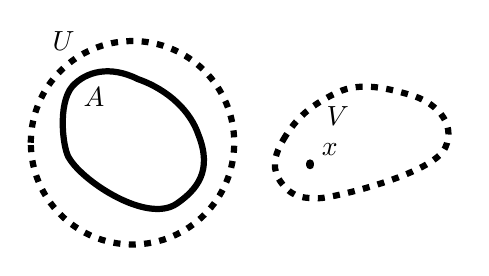
\begin{tikzpicture}[x=0.75pt,y=0.75pt,yscale=-0.75,xscale=0.75]
%uncomment if require: \path (0,300); %set diagram left start at 0, and has height of 300

%Shape: Polygon Curved [id:ds7476061327261551] 
\draw  [line width=2.25] [line join = round][line cap = round] (183.79,131.76) .. controls (165.79,122.76) and (150.48,126.87) .. (141.8,136.27) .. controls (131.79,147.76) and (135.79,177.76) .. (139.79,182.76) .. controls (148.79,197.76) and (189.79,224.76) .. (208.79,211.76) .. controls (221.79,202.76) and (231.79,190.76) .. (222.79,167.76) .. controls (217.79,152.76) and (203.79,138.76) .. (183.79,131.76) -- cycle ;
%Shape: Circle [id:dp8494851000309646] 
\draw  [dash pattern={on 2.53pt off 3.02pt}][line width=2.25]  (115,172.65) .. controls (115,136.56) and (144.26,107.31) .. (180.35,107.31) .. controls (216.44,107.31) and (245.69,136.56) .. (245.69,172.65) .. controls (245.69,208.74) and (216.44,238) .. (180.35,238) .. controls (144.26,238) and (115,208.74) .. (115,172.65) -- cycle ;
%Shape: Regular Polygon [id:dp01574201056466351] 
\draw  [dash pattern={on 2.53pt off 3.02pt}][line width=2.25]  (278.68,168.31) .. controls (270.59,181.22) and (269.18,189.93) .. (276.68,199.31) .. controls (284.18,208.68) and (291.57,208.11) .. (299.68,208.31) .. controls (307.79,208.5) and (373.17,193) .. (381.17,176) .. controls (389.17,159) and (373.17,146) .. (359.17,142) .. controls (345.17,138) and (327.17,133) .. (311.78,140.39) .. controls (296.38,147.78) and (286.78,155.39) .. (278.68,168.31) -- cycle ;
%Shape: Free Drawing [id:dp4390180870472238] 
\draw  [line width=3] [line join = round][line cap = round] (294.5,187) .. controls (294.5,186.67) and (294.5,186.33) .. (294.5,186) ;

% Text Node
\draw (147,135.4) node [anchor=north west][inner sep=0.75pt]    {$A$};
% Text Node
\draw (127,99.4) node [anchor=north west][inner sep=0.75pt]    {$U$};
% Text Node
\draw (300,171.4) node [anchor=north west][inner sep=0.75pt]    {$x$};
% Text Node
\draw (303,147.4) node [anchor=north west][inner sep=0.75pt]    {$V$};


\end{tikzpicture}
\caption{proposition \ref{8.8.10}}
    \end{figure}
\end{proofenv}
\begin{corollaryenv}
    Let $(X,\mathscr{T})$ be a Hausdorff topological space, and $A$ and $B$ be disjoint compact subset of $X$. There exist $(U,V)\in\mathscr{T}^2$, such that $A\subseteq U$, $B\subseteq V$ and $U\cap V=\varnothing$.
\end{corollaryenv}
\begin{proofenv}
    By (1) of the previous proposition.
    $$\forall x\in B,\ \exists (U_x, V_x)\in \mathscr{T}^2,\ A\subseteq U_x,\ x\in V_x,\ U_x\cap V_x=\varnothing.$$
    $B\subseteq \bigcup_{x\in B}V_x.$ So, $\exists \{x_1,\ldots,x_n\}\subseteq B$, such that $\dis B\subseteq \bigcup_{i=1}^n V_{x_i}$. Let
    $$U=\bigcap_{i=1}^nU_{x_i}\in \mathscr{T},\ V=\bigcup_{i=1}^nV_{x_i}\in \mathscr{T}.$$
    Then, $A\subseteq U$, $B\subseteq V$, and $U\cap V=\varnothing$.
\end{proofenv}
\begin{theoremenv}
    Let $(X,\mathscr{T})$ be a topological space and $A$ be a compact subset of $X$. Let $(I,\le)$ be a partially ordered set and $(F_i)_{i\in I}$ be a decreasing family of closed subsets of $X$. Assume that, any finite subset of $I$ has an upper bound in $I$. If $\dis \left(\bigcap_{i\in I}F_i\right)\cap A=\varnothing$, then exists $i_0\in I$ such that $F_{i_0}\cap A=\varnothing$.
\end{theoremenv}
\begin{remark}
    In the particular case where $I=\mathbb{N}$, the theorem becomes: If $(A_n)_{n\in \NN}$ is a sequence of compact non-empty subsets of $X$ such that $A_0\supseteq A_1\supseteq A_2\supseteq\cdots$, then $\dis\bigcap_{n\in \NN}A_n\neq\varnothing$. 
\end{remark}
\begin{proofenv}
    $\forall i\in I$, let $U_i=X\backslash F_i\in \mathscr{T}$. Since $\dis \left(\bigcap_{i\in I}F_i\right)\cap A=\varnothing$. $\dis A\subseteq X\backslash \bigcap_{i\in I}F_i=\bigcup_{i\in I}U_i$.
    Since $A$ is compact, $\exists J\subseteq I$, finite such that $\dis A\subseteq \bigcup_{j\in J}U_j$. Let $i_0$ be an upper bound of $J$. $\forall j\in J$, $j\le i_0$. So $F_j\supset F_{i_0}$. $U_j\subseteq U_{i_0}$. Hence $A\subseteq U_{i_0}$, $A\cap F_{i_0}=\varnothing$.
\end{proofenv}
\begin{theoremenv}[Tychonoff]
    Let $I$ be a non-empty set and $(X_i,\mathscr{T}_i)$, $i\in I$ be topological spaces. Let $\dis X=\prod_{i\in I}X_i$, and $\mathscr{T}$ be the product topology of $\left(\mathscr{T}_i\right)_{i\in I}$. For any $i\in I$, let $A_i$ be a compact subset of $X_i$, let $\dis A=\prod_{i\in I}A_i \subseteq X$. Then $A$ is compact subset of $X$.
    
\end{theoremenv}
\begin{proofenv}
    For any $i\in I$, let $\pi_i: (x_j)_{j\in I}\longmapsto x_i$ be the projection mapping. 
    $$A=\bigcap_{i\in I}\pi^{-1}_{i}(A_i).$$
    Let $\mathcal{F}$ be an ultrafilter on $X$ such that $A\in \mathcal{F}$. Then $\forall i\in I$, $\pi_{i*}(\mathcal{F})=:\mathcal{F}_i$ is an ultrafilter on $X_i$ such that $A_i\in \mathcal{F}_i$. Since $A_i$ is compact, $\mathcal{F}_i$ has a limit point $x_i\in A_i$. Let $x=(x_i)_{i\in I}$. Let $U$ be a neighborhood of $x$. There exists $J\subseteq I$ finite and $U_j\in J_j\ (j\in J)$ such that $x_j\in U_j$ and $\dis \bigcap_{j\in J}\pi_{j}^{-1}(U_j)\subseteq U$. $\forall j\in J, U_j\in \mathcal{F}_j$. Since $x_j$ is a limit point of $\mathcal{F}_j$. Hence $\pi^{-1}_j(U_j)\in \mathcal{F}$. Thus $\dis \bigcap_{j\in J}\pi_{j}^{-1}(U_j)\in \mathcal{F}$, which implies $U\in \mathcal{F}$. 
\end{proofenv}

\newpage
\section{Compact Metric Spaces}
\begin{definitionenv}
    Let $(X,\mathscr{T})$ be a topological space and $Y\subseteq X$. If any sequence in $Y$ has a subsequence that converges to some element of $X$. We say that $Y$ is \textbf{sequentially compact}.
\end{definitionenv}
\begin{theoremenv}
    Let $(X,\mathscr{T})$ be a topological space and $Y\subseteq X$. If $Y$ is compact and if each $y\in Y$ has a countable neighborhood basis, then $Y$ is sequentially compact.
\end{theoremenv}
\begin{proofenv}
    Let $x=(x_n)_{n\in I}$ be a sequence in $Y$ and $\mathcal{F}$ be the Fréchet filter of $I$. Then $x_*(\mathcal{F})$ is a non-degenerate filter on $X$ and $Y\in x_*(\mathcal{F})$. Since $Y$ is compact, $x_*(\mathcal{F})$ has an adherent point $p\in Y$. Let $(U_k)_{k\in \NN}$ be a decreasing sequence of neighborhood of $p$ such that $\{U_k\mid k\in \NN\}$ forms a neighborhood basis of $p$. Therefore we can construct in a recursive way  a strictly increasing sequence $(n_k)_{k\in \NN} $ in $I$ such that $x_{n_k}\in U_k$. Thus $(x_{n_k})_{k\in \NN}$ converges to $p$.
\end{proofenv}
\begin{theoremenv}
    Let $(X,\dd)$ be a metric space, and $Y\subseteq X$. The following conditions are equivalent:
    \newline
    (1) $Y$ is compact.
    \newline
    (2) $(Y,\dd)$ is complete and
    $$\forall \varepsilon>0,\ \exists A_\varepsilon\subseteq Y\text{ finite},\ Y\subseteq \bigcup_{x\in A_\varepsilon}B(x,\varepsilon).  $$
    \newline
    (3) $Y$ is sequentially compact.
\end{theoremenv}
\begin{proofenv}
    \ \newline
    (1)$\Rightarrow$ (2) Let $\mathcal{F}$ be a Cauchy filter on $Y$. Let $f:Y\longrightarrow X$ be the inclusion mapping. Then $f_*(\mathcal{F})$ is a Cauchy filter on $X$ and $Y\in f_*(\mathcal{F})$. Since $Y$ is compact, $f_*(\mathcal{F})$ has an adherent point $l\in Y$. So $l$ is a limit point of $f_*(\mathcal{F})$ (since $f_*(\mathcal{F})$ is a Cauchy filter.) For any $U\in V_{l}(\mathscr{T})$, $U\in f_*(\mathcal{F})$, namely, $f^{-1}(U)=U\cap Y\in \mathcal{F}$. Thus $l$ is a limit point of $\mathcal{F}$. Since $Y\subseteq \bigcup_{y\in Y}B(y,\varepsilon)$. Since $Y$ is compact, $\exists A_\varepsilon\subseteq Y$ finite, such that $\dis Y\subseteq \bigcup_{x\in A_\varepsilon}B(x,\varepsilon)$.
    \newline
    (2)$\Rightarrow$ (1) Let $\mathcal{F}$ be an ultrafilter on $X$ such that $Y\in \mathcal{F}$. For any $\varepsilon>0$, $\dis\bigcup_{x\in A_\varepsilon}B(x,\varepsilon)\in \mathcal{F}$. Hence $\mathcal{F}$ is a Cauchy filter, which implies that $\mathcal{F}|_Y\coloneq\{Y\cap U\mid U\in \mathcal{F}\}$ is a Cauchy filter. Thus $\mathcal{F}|_Y$ has a limit point $l\in Y$, which is also a limit point of $\mathcal{F}$.
    \newline
    (2)$\Rightarrow$ (3) is already known.
    \newline
    (3)$\Rightarrow$ (1) Let $(x_n)_{n\in I}$ be a Cauchy sequence in $Y$. Since $Y$ is sequentially compact, $(x_n)_{n\in I}$ has a subsequence that converges to some $l\in Y$. Since $(x_n)_{n\in I}$ is a Cauchy sequence, it converges to $l$. We prove the second statement by contradiction. 
    
    \quad Assume that $\varepsilon>0$ is such that $Y$ cannot be covered by finitely many balls centered in $Y$ with radius $\varepsilon$. We construct recursively a sequence $(x_n)_{n\in\NN}$ as follows. $x_0\in Y$ is chosen arbitrarily. If $x_0,\ldots,x_n$ are chosen, we pick 
    $$x_{n+1}\in Y\backslash \bigcup_{i=0}^{n}B(x_i,\varepsilon).$$
    Then $\forall(i,j)\in \NN^2, i\neq j, \dd(x_i,x_j)<\varepsilon$. So $(x_n)_{n\in \NN}$ does not have any Cauchy subsequence. It cannot have a convergent subsequence.
\end{proofenv}
\begin{exampleenv}
    Let $(a,b)\in \RR^2$, $a<b$. $\interval{a}{b}$ is closed. $\forall \varepsilon, \exists N\in \NN_{>0}$. $\frac{b-a}{N}<\varepsilon$. $\forall i\in \{0,\ldots, N\}$, let $x_i=a+\frac{i}{N}(b-a)$. $a=x_0<x_1<\cdots<x_{N-1}<x_N=b$. 
    $$[a,b]\subseteq\bigcup_{i=0}^{N}B(x_i,\varepsilon)=\bigcup_{i=0}^{n}\interval[open]{x_i-\varepsilon}{x_{i}+\varepsilon}.$$
    So $[a,b]$ is compact.
\end{exampleenv}
\begin{propositionenv}
    Let $(X,\dd)$ be a metric space and $Y\subseteq X$. If $Y$ is compact, then $Y$ is bounded and closed.
\end{propositionenv}
\begin{proofenv}
    Since $X$ is Hausdorff, $Y$ is closed. $\exists A\subseteq Y$ finite, $Y\subseteq \bigcup_{x\in A}B(x,1)$. Since each $B(x,1)$ is bounded, so is $Y$.
\end{proofenv}
\begin{definitionenv}
    Let $(X,\mathscr{T})$ be a topological space. If $\forall x\in X$, $x$ has a compact neighborhood, we say that $X$ is \textbf{locally compact}.
\end{definitionenv}
\begin{exampleenv}
    $(\RR),\left|\ \cdot\ \right|$ is locally compact. 
    $$\forall x\in \RR, [x-1,x+1] \text{ is compact neighborhood of } x.$$
\end{exampleenv}
\begin{propositionenv}
    Let $(K,\left|\ \cdot\ \right|)$ be a locally compact valued field. Then,
    \newline
    (1) $(K,\left|\ \cdot\ \right|)$ is complete.
    \newline
    (2) Assume that exists $a\in K$, $|a|>1$. Let $(V,\pl\cdot\pl)$ be a finite-dimensional vector space over $K$. Then any bounded closed subset of $V$ is compact.
    \newline
    (3) $(V,\pl\cdot\pl)$  is locally compact.
\end{propositionenv}
\begin{proofenv}
    \ \newline
    (2) Assume that $V=K^n$, $\pl(a_1,\ldots,a_n)\pl=\max\{|a_1|,\ldots,|a_n|\}.$ Let $A\subseteq K^n$, bounded, closed. Let $R>0$, $A\subseteq \bar{B}(0_V,R)$. 

    \quad Since $(K,\left|\ \cdot\ \right|)$ is locally compact, there exists a compact neighborhood $U$ of $0_K\in K$. $\exists\varepsilon>0, \bar{B}(0,\varepsilon)\subseteq U$. So $\bar{B}(0_K,\varepsilon)$ is compact. Take $n\in \NN_{\ge 1}$ such that $|a|^n\varepsilon> R$.
    $$f:K\longrightarrow K \text{continuous}$$
    $$b\longmapsto a^n b$$
    $f\left(\bar{B}(0_K,\varepsilon)\right)=a^n\bar{B}(0_K,\varepsilon)\supseteq \bar{B}(0_K,R).$ is compact. By Tychonoff theorem, $\bar{B}(0_V,R)$ is compact. Since $A$ is closed, $A$ is compact.
    \newline
    (3) $\bar{B}(0_V,R)$ is compact for any $R>0$.
    \newline
    (1) $B(0_K,R)$ is compact for any $R>0$. For any Cauchy sequence $(a_n)_{n\in \NN}$ in $K$, $\exists R>0$. $\{a_n\mid n\in \NN\}\subseteq \bar{B}(0_K,R)$, so $(a_n)_{n\in \NN}$ converges.
\end{proofenv}
\begin{lemmaenv}
    Let $A\subseteq R$ be a non-empty compact subset. Then $A$ has a greatest and least element.
\end{lemmaenv}
\begin{proofenv}
    Since $A$ is non-empty and bounded, $\{\sup A,\inf A\}\subseteq \RR$. Since $A=\bar{A}$, $\sup A\in A, \inf A\in A$.
\end{proofenv}
\begin{theoremenv}
    Let $(X,\mathscr{T})$ be a topological space and $f:X\longrightarrow \RR$ be a continuous mapping. If $Y\subseteq X$ is compact, then $f|_Y$ has its maximum and minimum. ($\exists x_1\in Y, f(x_1)\ge f(y), \forall y\in Y$. $\exists x_2\in Y,\forall y\in Y, f(x_2)\le f(y)$.)
\end{theoremenv}
\begin{proofenv}
    $f(Y)\subseteq \RR\text{ is compact.}$
\end{proofenv}
\begin{theoremenv}
    Let $(X,\dd_X)$ and $(Y,\dd_Y)$ be metric spaces, $f:X\longrightarrow Y$ be a continuous mapping. If $(X,\dd_X)$ is compact, then $f$ is uniformly continuous.
\end{theoremenv}
\begin{proofenv}
    $f$ is uniformly continuous if and only if 
    $$\forall \varepsilon>0,\ \exists \delta>0,\ \forall x,y\in X,\ \dd_X(x,y)<\delta \Rightarrow \dd_Y(f(x),f(y))<\varepsilon.$$
    Suppose by contradiction that $f$ is not uniformly continuous. That is 
    $$\exists \varepsilon>0,\ \forall \delta>0,\ \exists (x_1,x_2)\in X^2,\ \dd_X(x_1,x_2)<\delta \text{ and } \dd_Y(f(x_1),f(x_2))\ge \varepsilon.$$
    So we can choose sequences $(x_n)_{n\in \NN_{\ge1}}$ and $(y_n)_{n\in \NN_{\ge1}}$ in $X$ such that
    $$\forall n\in \NN, \dd_{X}(x_n,y_n)\le \frac{1}{n},\ \dd_Y(f(x_n),f(y_n))\ge \varepsilon.$$
    By compactness of $X$, there exists a subsequence $I\subseteq \NN_{\ge 1}$ finite, such that $(x_n)_{n\in I}$ converges to some $a\in X$, and $(y_n)_{n\in I}$ converges to some $b\in X$. Since $\dd_X:X\times X\longrightarrow \RR_{\ge 0}$ is continuous, 
    $$0\le \dd_{X}(a,b)=\lim_{n\in I,n\rightarrow+\infty}\dd_{X}(x_n,y_n)\le \lim_{n\in I,n\rightarrow+\infty}\frac{1}{n}.$$
\end{proofenv}

\newpage
\section{Path Connectedness}
\begin{definitionenv}
    Let $(X,\mathscr{T})$ be a topological space and $C$ be a subset of $X$. If for any $(x,y)\in C\times C$, there exists a continuous mapping $\varphi: [0,1]\longrightarrow C$, such that $\varphi(0)=x$ and $\varphi(1)=y$, we say that $C$ is \textbf{path connected}.

    \begin{figure}[H]
        \centering


\tikzset{every picture/.style={line width=0.75pt}} %set default line width to 0.75pt        

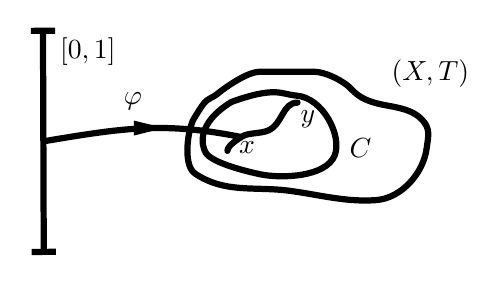
\begin{tikzpicture}[x=0.75pt,y=0.75pt,yscale=-0.75,xscale=0.75]
%uncomment if require: \path (0,300); %set diagram left start at 0, and has height of 300

%Straight Lines [id:da4419444137553179] 
\draw [line width=2.25]    (120,104) -- (120.5,246) ;
\draw [shift={(120.5,246)}, rotate = 269.8] [color={rgb, 255:red, 0; green, 0; blue, 0 }  ][line width=2.25]    (0,7.83) -- (0,-7.83)   ;
\draw [shift={(120,104)}, rotate = 269.8] [color={rgb, 255:red, 0; green, 0; blue, 0 }  ][line width=2.25]    (0,7.83) -- (0,-7.83)   ;
%Shape: Regular Polygon [id:dp4361348822258063] 
\draw  [line width=2.25]  (292.77,130.33) .. controls (281.5,130.33) and (270.23,130.12) .. (258.96,130.33) .. controls (251.27,130.47) and (237.48,139.96) .. (231.91,144.63) .. controls (229.41,146.73) and (225.86,147.55) .. (223.8,150.08) .. controls (221.21,153.24) and (219.2,156.83) .. (217.03,160.3) .. controls (213.2,166.42) and (209.44,190.16) .. (217.71,195.71) .. controls (236.61,208.41) and (255.93,203.93) .. (277.22,206.61) .. controls (296.7,209.07) and (314.22,214.2) .. (334.02,212.74) .. controls (350.44,211.53) and (364.51,195.23) .. (366.48,179.37) .. controls (367.22,173.45) and (368.9,168.09) .. (365.13,163.02) .. controls (357.39,152.62) and (343.57,153.37) .. (332.67,150.08) .. controls (324,147.46) and (321.35,144.81) .. (316.44,139.86) .. controls (314.23,137.64) and (302.2,129.76) .. (292.77,130.33) -- cycle ;
%Curve Lines [id:da285151310243584] 
\draw [line width=2.25]    (120.25,175) .. controls (173.5,166) and (198.5,162.44) .. (248.5,172.44) ;
\draw [shift={(197.67,166.44)}, rotate = 179.99] [fill={rgb, 255:red, 0; green, 0; blue, 0 }  ][line width=0.08]  [draw opacity=0] (19.2,-4.8) -- (0,0) -- (19.2,4.8) -- cycle    ;
%Shape: Regular Polygon [id:dp12922208257094558] 
\draw  [line width=2.25]  (241.1,149.67) .. controls (218.3,163.62) and (221.84,177.72) .. (224.52,182.23) .. controls (228.41,188.79) and (250.24,194.19) .. (259.75,196.19) .. controls (272.85,198.94) and (301.83,198.1) .. (307.42,183.98) .. controls (312.32,171.6) and (299.94,146.81) .. (282.55,145.59) .. controls (273.49,144.96) and (270.11,139.2) .. (241.1,149.67) -- cycle ;
%Shape: Free Drawing [id:dp6548439894976998] 
\draw  [line width=2.25] [line join = round][line cap = round] (238.5,181.11) .. controls (238.5,177.77) and (245.34,173.54) .. (247.5,172.11) .. controls (251.79,169.25) and (259.06,170.28) .. (264.5,168.11) .. controls (273.94,164.33) and (273.63,150.11) .. (283.5,150.11) ;

% Text Node
\draw (129,106.4) node [anchor=north west][inner sep=0.75pt]    {$[ 0,1]$};
% Text Node
\draw (342,120.4) node [anchor=north west][inner sep=0.75pt]    {$( X,\mathscr{T})$};
% Text Node
\draw (170,141.4) node [anchor=north west][inner sep=0.75pt]    {$\varphi $};
% Text Node
\draw (244,173.4) node [anchor=north west][inner sep=0.75pt]    {$x$};
% Text Node
\draw (283.55,152.99) node [anchor=north west][inner sep=0.75pt]    {$y$};
% Text Node
\draw (315,171.4) node [anchor=north west][inner sep=0.75pt]    {$C$};


\end{tikzpicture}
\caption{Path connected}
    \end{figure}
\end{definitionenv}

\begin{propositionenv}
    Let $(X,\mathscr{T}_X)$, $(Y,\mathscr{T}_Y)$ be two topological spaces and $f:X\longrightarrow Y$ be continuous mapping. If $C\subseteq X$ is path connected, then $f(C)\subseteq Y$ is path connected.
\end{propositionenv}
\begin{proofenv}
    Let $(a,b)\in C\times C$. There exist $(x,y)\in C\times C$ such that $f(x)=a$ and $f(y)=b$. Since $C$ is path connected, so we have a continuous $\varphi: [0,1]\longrightarrow C$ such that $\varphi(0)=x$ and $\varphi(1)=y$. Then $f\circ \varphi: [0,1]\longrightarrow f(C)$ is continuous, and 
    $$\left(f\circ\varphi\right)(0)=f(x)=a,\ \left(f\circ\varphi\right)(1)=f(y)=b.$$
    Hence $f(C)$ is path connected.
\end{proofenv}
\begin{theoremenv}
    Let $I$ be a subset of $\RR$. $I$ is path connected if and only if $I$ is an interval.
\end{theoremenv}
\begin{proofenv}
    \ \newline
    $\Leftarrow$ Assume that $I$ is an interval. Let $(a,b)\in I\times I$ such that $a\le b$. One has $[a,b]\subseteq I$. Consider $\varphi:[0,1]\longrightarrow I$ defined as:
    $$\varphi(t)=\frac{a+b}{2}+\frac{b-a}{2}t,\ t\in [0,1].$$
    This is the sum of a constant mapping and a linear mapping. Hence $\varphi$ is continuous. So $I$ is path connected.
    \newline
    $\Rightarrow$ Assume that $I$ is path connected. Let $(a,b)\in I\times I$, $a\le b$, $\varphi :[0,1]\longrightarrow I$ a continuous mapping such that $\varphi(0)=a$ and $\varphi(1)=b$. Let $c\in [a,b]$. It is suffices to show that $c\in I$. Assume that $c\notin I$. We have $a<c<b$. We will define two sequences $(x_n)_{n\in \NN}$, $(y_n)_{n\in \NN}$ in a recursive way: $x_0=0, y_0=1$. We want to have $\varphi(x_n)<\varphi(y_n)$. Let $(z_n)\coloneq \frac{x_n+y_n}{2}$.
    $$\begin{cases}
        x_{n+1}=x_n, y_{n+1}=z_n,\ \text{if }\varphi(z_n)>c,\\
        x_{n+1}=z_n, y_{n+1}=y_n,\ \text{if }\varphi(z_n)<c.
    \end{cases}$$
    Then the sequence $(x_n)_{n\in \NN}$ is increasing, $(y_n)_{n\in\NN}$ is decreasing, and $0\le y_n-x_n\le \frac{1}{2^n}$. So $(x_n)_{n\in\NN}$, $(y_n)_{n\in\NN}$ converge to the same point $d\in [0,1]$. Note that 
    $$\forall n\in \NN,\ \left(c-\varphi(x_n)\right)\left(c-\varphi(y_n)\right)<0.$$
    $$0\le \left(c-\varphi(d)\right)^2=\lim_{n\rightarrow \infty}\left(c-\varphi(x_n)\right)\left(c-\varphi(y_n)\right)\le0.$$
    So, $\varphi(d)=c$. Contradiction.
\end{proofenv}
\begin{corollaryenv}
    Let $I$ be an interval in $\RR$. If $f:I\longrightarrow R$ is a continuous mapping, then $f(I)$ is also an interval. In particular, if $f$ has a positive value and a negative value, then it must have a zero.
\end{corollaryenv}
\begin{proofenv}
    Since $I$ is path connected, so $f(I)$ is path connected. Hence $f(I)\subseteq \RR$ is an interval.
\end{proofenv}
